% !TeX spellcheck = en-US
% !TeX encoding = utf8
% !TeX program = pdflatex
% !BIB program = biber
% -*- coding:utf-8 mod:LaTeX -*-


% vv  scroll down to line 200 for content  vv


\let\ifdeutsch\iffalse
\let\ifenglish\iftrue


% EN: This file is loaded before the \documentclass command in the main document

% EN: The following package allows \\ at the title page
%     For more information see https://github.com/latextemplates/scientific-thesis-cover/issues/4
\RequirePackage{kvoptions-patch}

\ifenglish
  \PassOptionsToClass{numbers=noenddot}{scrbook}
\else
  %()Aus scrguide.pdf - der Dokumentation von KOMA-Script)
  %Nach DUDEN steht in Gliederungen, in denen ausschließlich arabische Ziffern für die Nummerierung
  %verwendet werden, am Ende der Gliederungsnummern kein abschließender Punkt
  %(siehe [DUD96, R3]). Wird hingegen innerhalb der Gliederung auch mit römischen Zahlen
  %oder Groß- oder Kleinbuchstaben gearbeitet, so steht am Ende aller Gliederungsnummern ein
  %abschließender Punkt (siehe [DUD96, R4])
  \PassOptionsToClass{numbers=autoendperiod}{scrbook}
\fi

% Warns about outdated packages and missing caption declarations
% See https://www.ctan.org/pkg/nag
\RequirePackage[l2tabu, orthodox]{nag}

%DE: Neue deutsche Trennmuster
%    Siehe http://www.ctan.org/pkg/dehyph-exptl und http://projekte.dante.de/Trennmuster/WebHome
%    Nur für pdflatex, nicht für lualatex
\RequirePackage{ifluatex}
\ifluatex
  % do not load anything
\else
  \ifdeutsch
    \RequirePackage[ngerman=ngerman-x-latest]{hyphsubst}
  \fi
\fi

\documentclass[
  %
  %ngerman, %%% Add if you write in German.
  %
  % fontsize=11pt is the standard
  a4paper,  % Standard format - only KOMAScript uses paper=a4 - https://tex.stackexchange.com/a/61044/9075
  twoside,  % we are optimizing for both screen and two-side printing. So the page numbers will jump, but the content is configured to stay in the middle (by using the geometry package)
  bibliography=totoc,
  %               idxtotoc,   %Index ins Inhaltsverzeichnis
  %               liststotoc, %List of X ins Inhaltsverzeichnis, mit liststotocnumbered werden die Abbildungsverzeichnisse nummeriert
  headsepline,
  cleardoublepage=empty,
  parskip=half,
  %               draft    % um zu sehen, wo noch nachgebessert werden muss - wichtig, da Bindungskorrektur mit drin
  draft=false
]{scrbook}
% !TeX encoding = utf8
% -*- coding:utf-8 mod:LaTeX -*-

% EN: This file includes basic packages and sets options. The order of package
%     loading is important

% DE: In dieser Datei werden zuerst die benoetigten Pakete eingebunden und
%     danach diverse Optionen gesetzt. Achtung Reihenfolge ist entscheidend!


% EN: Styleguide:
% - English comments are prefixed with "EN", German comments are prefixed with "DE"
% - Prefixed headings define the language for the subsequent paragraphs
% - It is tried to organize packages in blocks. Bocks are separated by two empty lines.

% DE: Styleguide:
%
% Ein sehr kleiner Styleguide. Packages werden in Blöcken organisiert.
% Zwischen zwei Blöcken sind 2 Leerzeilen!


% EN: Enable copy and paste of text from the PDF
%     Only required for pdflatex. It "just works" in the case of lualatex.
%     mmap enables mathematical symbols, but does not work with the newtx font set
%     See: https://tex.stackexchange.com/a/64457/9075
%     Other solutions outlined at http://goemonx.blogspot.de/2012/01/pdflatex-ligaturen-und-copynpaste.html and http://tex.stackexchange.com/questions/4397/make-ligatures-in-linux-libertine-copyable-and-searchable
%     Trouble shooting outlined at https://tex.stackexchange.com/a/100618/9075

\ifluatex
\else
  \usepackage{cmap}
\fi


% EN: File encoding
% DE: Codierung
%     Wir sind im 21 Jahrhundert, utf-8 löst so viele Probleme.
%
% Mit UTF-8 funktionieren folgende Pakete nicht mehr. Bitte beachten!
%   * fancyvrb mit §
%   * easylist -> http://www.ctan.org/tex-archive/macros/latex/contrib/easylist/
\ifluatex
  % EN: See https://tex.stackexchange.com/a/158517/9075
  %     Not required, because of usage of fontspec package
  %\usepackage[utf8]{luainputenc}
\else
  \usepackage[utf8]{inputenc}
\fi


% DE: Parallelbetrieb tex4ht und pdflatex

\makeatletter
\@ifpackageloaded{tex4ht}{
  \def\iftex4ht{\iftrue}
}{
  \def\iftex4ht{\iffalse}
}
\makeatother


% EN: Mathematics
% DE: Mathematik
%
% DE: Viele Mathematik-Sachen. Siehe https://texdoc.net/pkg/amsmath
%
% EN: Options must be passed this way, otherwise it does not work with glossaries
% DE: fleqn (=Gleichungen linksbündig platzieren) funktioniert nicht direkt. Es muss noch ein Patch gemacht werden:
\PassOptionsToPackage{fleqn,leqno}{amsmath}
%
% DE: amsmath Muss nicht mehr geladen werden, da es von newtxmath automatisch geladen wird
% \usepackage{amsmath}


%% EN: Fonts
%% DE: Schriften
%%
%% !!! If you change the font, be sure that words such as "workflow" can
%% !!! still be copied from the PDF. If this is not the case, you have
%% !!! to use glyphtounicode. See comment at cmap package


% EN: Times Roman for all text
\ifluatex
  % source: Second proposed fix from the following answer: https://tex.stackexchange.com/a/394137
  \usepackage[no-math]{fontspec}
  \setmainfont{TeXGyreTermes-Regular}[
       BoldFont       = TeXGyreTermes-Bold ,
       ItalicFont     = TeXGyreTermes-Italic ,
       BoldItalicFont = TeXGyreTermes-BoldItalic,
       NFSSFamily     = ntxtlf]
  \setsansfont{TeX Gyre Heros Regular}[
       Scale=.9,
       BoldFont       = TeX Gyre Heros Bold,
       ItalicFont     = TeX Gyre Heros Italic,
       BoldItalicFont = TeX Gyre Heros BoldItalic]
  \setmonofont[StylisticSet={1,3},Scale=.9]{inconsolata}
  \RequirePackage{newtxmath}
\else
  \RequirePackage{newtxtext}
  \RequirePackage{newtxmath}
  % EN: looks good with times, but no equivalent for lualatex found,
  %     therefore replaced with inconsolata
  %\RequirePackage[zerostyle=b,scaled=.9]{newtxtt}
  \RequirePackage[varl,scaled=.9]{inconsolata}
\fi

% EN: Fallback font - if the subsequent font packages do not define a font (e.g., monospaced)
%     This is the modern package for "Computer Modern".
%     In case this gets activated, one has to switch from cmap package to glyphtounicode (in the case of pdflatex)
% DE: Fallback-Schriftart
%\usepackage[%
%    rm={oldstyle=false,proportional=true},%
%    sf={oldstyle=false,proportional=true},%
%    tt={oldstyle=false,proportional=true,variable=true},%
%    qt=false%
%]{cfr-lm}

% EN: Headings are typset in Helvetica (which is similar to Arial)
% DE: Schriftart fuer die Ueberschriften - ueberschreibt lmodern
%\usepackage[scaled=.95]{helvet}

% DE: Für Schreibschrift würde tun, muss aber nicht
%\usepackage{mathrsfs} %  \mathscr{ABC}

% EN: Font for the main text
% DE: Schriftart fuer den Fliesstext - ueberschreibt lmodern
%     Linux Libertine, siehe http://www.linuxlibertine.org/
%     Packageparamter [osf] = Minuskel-Ziffern
%     rm = libertine im Brottext, Linux Biolinum NICHT als serifenlose Schrift, sondern helvet (von oben) beibehalten
%\usepackage[rm]{libertine}

% EN: Alternative Font: Palantino. It is recommeded by Prof. Ludewig for German texts
% DE: Alternative Schriftart: Palantino, Packageparamter [osf] = Minuskel-Ziffern
%     Bitte nur in deutschen Texten
%\usepackage{mathpazo} %ftp://ftp.dante.de/tex-archive/fonts/mathpazo/ - Tipp aus DE-TEX-FAQ 8.2.1

% DE: Schriftart fuer Programmcode - ueberschreibt lmodern
%     Falls auskommentiert, wird die Standardschriftart lmodern genommen
%     Fuer schreibmaschinenartige Schluesselwoerter in den Listings - geht bei alten Installationen nicht, da einige Fontshapes (<>=) fehlen
%\usepackage[scaled=.92]{luximono}
%\usepackage{courier}
% DE: BeraMono als Typewriter-Schrift, Tipp von http://tex.stackexchange.com/a/71346/9075
%\usepackage[scaled=0.83]{beramono}

% EN: backticks (`) are rendered as such in verbatim environments.
%     See following links for details:
%     - https://tex.stackexchange.com/a/341057/9075
%     - https://tex.stackexchange.com/a/47451/9075
%     - https://tex.stackexchange.com/a/166791/9075
\usepackage{upquote}

% DE: Symbole
%
%\usepackage[geometry]{ifsym} % \BigSquare
%\usepackage{mathabx}
%\usepackage{stmaryrd} %fuer \ovee, \owedge, \otimes
%\usepackage{marvosym} %fuer \Writinghand %patched to not redefine \Rightarrow
%\usepackage{mathrsfs} %mittels \mathscr{} schoenen geschwungenen Buchstaben erzeugen
%\usepackage{calrsfs} %\mathcal{} ein bisserl dickeren buchstaben erzeugen - sieht net so gut aus.
%durch mathpazo ist das schon definiert

%
%\usepackage{amssymb}

% EN: For \texttrademark{}
\usepackage{textcomp}

% EN: name-clashes von marvosym und mathabx vermeiden:
\def\delsym#1{%
  %  \expandafter\let\expandafter\origsym\expandafter=\csname#1\endcsname
  %  \expandafter\let\csname orig#1\endcsname=\origsym
  \expandafter\let\csname#1\endcsname=\relax
}

%\usepackage{pifont}
%\usepackage{bbding}
%\delsym{Asterisk}
%\delsym{Sun}\delsym{Mercury}\delsym{Venus}\delsym{Earth}\delsym{Mars}
%\delsym{Jupiter}\delsym{Saturn}\delsym{Uranus}\delsym{Neptune}
%\delsym{Pluto}\delsym{Aries}\delsym{Taurus}\delsym{Gemini}
%\delsym{Rightarrow}
%\usepackage{mathabx} - Ueberschreibt leider zu viel - und die \le-Zeichen usw. sehen nicht gut aus!


% EN: Modern font encoding
%     Has to be loaded AFTER any font packages. See https://tex.stackexchange.com/a/2869/9075.
\ifluatex
\else
  \usepackage[T1]{fontenc}
\fi
%


% EN: Character protrusion and font expansion. See http://www.ctan.org/tex-archive/macros/latex/contrib/microtype/
% DE: Optischer Randausgleich und Grauwertkorrektur

\usepackage[
  babel=true, % EN: Enable language-specific kerning. Take language-settings from the languge of the current document (see Section 6 of microtype.pdf)
  expansion=alltext,
  protrusion=alltext-nott, % EN: Ensure that at listings, there is no change at the margin of the listing
  final % EN: Always enable microtype, even if in draft mode. This helps finding bad boxes quickly.
        %     In the standard configuration, this template is always in the final mode, so this option only makes a difference if "pros" use the draft mode
]{microtype}


% EN: \texttt{test -- test} keeps the "--" as "--" (and does not convert it to an en dash)
\DisableLigatures{encoding = T1, family = tt* }

% DE: fuer microtype
% DE: tracking=true muss als Parameter des microtype-packages mitgegeben werden
% DE: Deaktiviert, da dies bei Algorithmen seltsam aussieht

%\DeclareMicrotypeSet*[tracking]{my}{ font = */*/*/sc/* }%
%\SetTracking{ encoding = *, shape = sc }{ 45 }
% DE: Hier wird festgelegt,
%     dass alle Passagen in Kapitälchen automatisch leicht
%     gesperrt werden.
%     Quelle: http://homepage.ruhr-uni-bochum.de/Georg.Verweyen/pakete.html
%    Deaktiviert, da sonst "BPEL", "BPMN" usw. wirklich komisch aussehen.
%     Macht wohl nur bei geisteswissenschaftlichen Arbeiten Sinn.


% EN: amsmath teaks


% EN: Fixes bugs in AMS math
%     Corrently conflicts with unicode-math
% \usepackage{mathtools}

%\numberwithin{equation}{section}
%\renewcommand{\theequation}{\thesection.\Roman{equation}}

% EN: work-around ams-math problem with align and 9 -> 10. Does not work with glossaries, No visual changes.
%\addtolength\mathindent{1em}


% EN: For theorems, replacement for amsthm
\usepackage[amsmath,hyperref]{ntheorem}
\theorempreskipamount 2ex plus1ex minus0.5ex
\theorempostskipamount 2ex plus1ex minus0.5ex
\theoremstyle{break}
\newtheorem{definition}{Definition}[section]


% CTAN: https://ctan.org/pkg/lccaps
% Doc: http://texdoc.net/pkg/lccaps
%
% Required for DE/EN \initialism
\usepackage{lccaps}


% EN: Defintion of colors. Argument "hyperref" is not used as we do not want to change border colors of links: Links are not colored anymore.
% DE: Farbdefinitionen
\usepackage[dvipsnames]{xcolor}


% EN: Required for custom acronyms/glossaries style.
%     Left aligned Columns in tables with fixed width.
%     See http://tex.stackexchange.com/questions/91566/syntax-similar-to-centering-for-right-and-left
\usepackage{ragged2e}


% DE: Wichtig, ansonsten erscheint "No room for a new \write"
\usepackage{scrwfile}


% EN: Support for language-specific hyphenation
% DE: Neue deutsche Rechtschreibung und Literatur statt "Literature"
%     Die folgende Einstellung ist der Nachfolger von ngerman.sty
\ifdeutsch
  % DE: letzte Sprache ist default, Einbindung von "american" ermöglicht \begin{otherlanguage}{amercian}...\end{otherlanguage} oder \foreignlanguage{american}{Text in American}
  %     Siehe auch http://tex.stackexchange.com/a/50638/9075
  \usepackage[american,main=ngerman]{babel}
  % Ein "abstract" ist eine "Kurzfassung", keine "Zusammenfassung"
  \addto\captionsngerman{%
    \renewcommand\abstractname{Kurzfassung}%
  }
  \ifluatex
    % EN: conditionally disable ligatures. See https://github.com/latextemplates/scientific-thesis-template/issues/54
    %     for a discussion
    \usepackage[ngerman]{selnolig}
  \fi
\else
  % EN: Set English as language and allow to write hyphenated"=words
  %     `american`, `english` and `USenglish` are synonyms for babel package (according to https://tex.stackexchange.com/questions/12775/babel-english-american-usenglish).
  %      "english" has to go last to set it as default language
  \usepackage[english]{babel}
  % EN: Hint by http://tex.stackexchange.com/a/321066/9075 -> enable "= as dashes
  \addto\extrasenglish{\languageshorthands{ngerman}\useshorthands{"}}
  \ifluatex
    % EN: conditionally disable ligatures. See https://github.com/latextemplates/scientific-thesis-template/issues/54
    %     for a discussion
    \usepackage[english]{selnolig}
  \fi
\fi
%


% EN: For easy quotations: \enquote{text}
%     This package is very smart when nesting is applied, otherwise textcmds (see below) provides a shorter command
%     Note that this package results in a warning when it is loaded before minted (actually fvextra).
% DE: Anführungszeichen
%     Zitate in \enquote{...} setzen, dann werden automatisch die richtigen Anführungszeichen verwendet.
%     Dieses package erzeugt eine Warnung, wenn es vor minted (genauer fvextra) geladen wird.
\usepackage{csquotes}


% EN: For even easier quotations: \qq{text}.
%     Is not smart in the case of nesting, but good enough for the most cases
\usepackage{textcmds}
\ifdeutsch
  % EN: German quotes are different. So do not use the English quotes, but the ones provided by the csquotes package.
  \renewcommand{\qq}[1]{\enquote{#1}}
\fi


% EN: extended enumarations
% DE: erweitertes Enumerate
\usepackage{paralist}


% DE: Gestaltung der Kopf- und Fußteilen

\usepackage[automark]{scrlayer-scrpage}

\automark[section]{chapter}
\setkomafont{pageheadfoot}{\normalfont\sffamily}
\setkomafont{pagenumber}{\normalfont\sffamily}

% DE: funktioniert nicht: Alle Linien sind hier weg
%\setheadsepline[.4pt]{.4pt}


% DE: Intelligentes Leerzeichen um hinter Abkürzungen die richtigen Abstände zu erhalten, auch leere.
%     Siehe commands.tex \gq{}
\usepackage{xspace}
% DE: Macht \xspace und \enquote kompatibel
\makeatletter
\xspaceaddexceptions{\grqq \grq \csq@qclose@i \} }
\makeatother


\newcommand{\eg}{e.\,g.,\ }
\newcommand{\ie}{i.\,e.,\ }


% EN: introduce \powerset - hint by http://matheplanet.com/matheplanet/nuke/html/viewtopic.php?topic=136492&post_id=997377
\DeclareFontFamily{U}{MnSymbolC}{}
\DeclareSymbolFont{MnSyC}{U}{MnSymbolC}{m}{n}
\DeclareFontShape{U}{MnSymbolC}{m}{n}{
  <-6>    MnSymbolC5
  <6-7>   MnSymbolC6
  <7-8>   MnSymbolC7
  <8-9>   MnSymbolC8
  <9-10>  MnSymbolC9
  <10-12> MnSymbolC10
  <12->   MnSymbolC12%
}{}
\DeclareMathSymbol{\powerset}{\mathord}{MnSyC}{180}


% EN: Package for the appendix
% DE: Anhang
\usepackage{appendix}
%[toc,page,title,header]
%


% EN: Graphics
% DE: Grafikeinbindungen
%
% EN: The parameter "pdftex" is not required
\usepackage{graphicx}
\graphicspath{{\getgraphicspath}}
\newcommand{\getgraphicspath}{graphics/}


% EN: Enables inclusion of SVG graphics - 1:1 approach
%    This is NOT the approach of https://ctan.org/pkg/svg-inkscape,
%     which allows text in SVG to be typeset using LaTeX
%     We just include the SVG as is.
\usepackage{epstopdf}
\epstopdfDeclareGraphicsRule{.svg}{pdf}{.pdf}{%
  inkscape -z -D --file=#1 --export-pdf=\OutputFile
}


% EN: Enables inclusion of SVG graphics - text-rendered-with-LaTeX-approach
%     This is the approach of https://ctan.org/pkg/svg-inkscape,
\newcommand{\executeiffilenewer}[3]{%
  \IfFileExists{#2}
  {
    %\message{file #2 exists}
    \ifnum\pdfstrcmp{\pdffilemoddate{#1}}%
      {\pdffilemoddate{#2}}>0%
      {\immediate\write18{#3}}
    \else
      {%\message{file up to date #2}
      }
    \fi%
  }{
    %\message{file #2 doesn't exist}
    %\message{argument: #3}
    %\immediate\write18{echo "test" > xoutput.txt}
    \immediate\write18{#3}
  }
}
\newcommand{\includesvg}[1]{%
  \executeiffilenewer{#1.svg}{#1.pdf}%
  {
    inkscape -z -D --file=\getgraphicspath#1.svg %
    --export-pdf=\getgraphicspath#1.pdf --export-latex}%
  \input{\getgraphicspath#1.pdf_tex}%
}


% EN: Enable typesetting values with SI units.
%\ifdeutsch
%  \usepackage[mode=text,group-four-digits]{siunitx}
%  \sisetup{locale=DE}
%\else
%  \usepackage[mode=text,group-four-digits,group-separator={,}]{siunitx}
%  \sisetup{locale=US}
%\fi


% EN: Extensions for tables
% DE: Tabellenerweiterungen
\usepackage{array} %increases tex's buffer size and enables ``>'' in tablespecs
\usepackage{longtable}
\usepackage{dcolumn} %Aligning numbers by decimal points in table columns
\ifdeutsch
  \newcolumntype{d}[1]{D{.}{,}{#1}}
\else
  \newcolumntype{d}[1]{D{.}{.}{#1}}
\fi
\setlength{\extrarowheight}{1pt}


% DE: Eine Zelle, die sich über mehrere Zeilen erstreckt.
%     Siehe Beispieltabelle in Kapitel 2
\usepackage{multirow}


% DE: Fuer Tabellen mit Variablen Spaltenbreiten
\usepackage{tabularx}
%\usepackage{tabulary}


% EN: Links behave as they should. Enables "\url{...}" for URL typesettings.
%     Allow URL breaks also at a hyphen, even though it might be confusing: Is the "-" part of the address or just a hyphen?
%     See https://tex.stackexchange.com/a/3034/9075.
% DE: Links verhalten sich so, wie sie sollen
%     Zeilenumbrüche bei URLs auch bei Bindestrichen erlauben, auch wenn es verwirrend sein könnte: Gehört der Bindestrich zur URL oder ist es ein Trennstrich?
%     Siehe https://tex.stackexchange.com/a/3034/9075.
\usepackage[hyphens]{url}
%
%  EN: When activated, use text font as url font, not the monospaced one.
%      For all options see https://tex.stackexchange.com/a/261435/9075.
% \urlstyle{same}
%
% EN: Hint by http://tex.stackexchange.com/a/10419/9075.
\makeatletter
\g@addto@macro{\UrlBreaks}{\UrlOrds}
\makeatother


% DE: Index über Begriffe, Abkürzungen
%\usepackage{makeidx} makeidx ist out -> http://xindy.sf.net verwenden


% DE: lustiger Hack fuer das Abkuerzungsverzeichnis
%     nach latex durchlauf folgendes ausfuehren
%     makeindex ausarbeitung.nlo -s nomencl.ist -o ausarbeitung.nls
%     danach nochmal latex
%\usepackage{nomencl}
%    \let\abk\nomenclature %Deutsche Ueberschrift setzen
%          \renewcommand{\nomname}{List of Abbreviations}
%        %Punkte zw. Abkuerzung und Erklaerung
%          \setlength{\nomlabelwidth}{.2\hsize}
%          \renewcommand{\nomlabel}[1]{#1 \dotfill}
%        %Zeilenabstaende verkleinern
%          \setlength{\nomitemsep}{-\parsep}
%    \makenomenclature


% EN: Logic for TeX - enables if-then-else in commands
% DE: Logik für TeX
%     FÜr if-then-else @ commands.tex
\usepackage{ifthen}


% EN: Code Listings
% DE: Listings
\usepackage{listings}
\lstset{language=XML,
  showstringspaces=false,
  extendedchars=true,
  basicstyle=\footnotesize\ttfamily,
  commentstyle=\slshape,
  % DE: Original: \rmfamily, damit werden die Strings im Quellcode hervorgehoben. Zusaetzlich evtl.: \scshape oder \rmfamily durch \ttfamily ersetzen. Dann sieht's aus, wie bei fancyvrb
  stringstyle=\ttfamily,
  breaklines=true,
  breakatwhitespace=true,
  % EN: alternative: fixed
  columns=flexible,
  numbers=left,
  numberstyle=\tiny,
  basewidth=.5em,
  xleftmargin=.5cm,
  % aboveskip=0mm, %DE: deaktivieren, falls man lstlistings direkt als floating object benutzt (\begin{lstlisting}[float,...])
  % belowskip=0mm, %DE: deaktivieren, falls man lstlistings direkt als floating object benutzt (\begin{lstlisting}[float,...])
  captionpos=b
}

\ifluatex
\else
  % EN: Enable UTF-8 support - see https://tex.stackexchange.com/q/419327/9075
  \usepackage{listingsutf8}
  \lstset{inputencoding=utf8/latin1}
\fi

\ifdeutsch
  \renewcommand{\lstlistlistingname}{Verzeichnis der Listings}
\fi


% EN: Alternative to listings could be fancyvrb. Can be used together.
% DE: Alternative zu Listings ist fancyvrb. Kann auch beides gleichzeitig benutzt werden.
\usepackage{fancyvrb}
%
% EN: Font size for the normal text
% DE: Groesse fuer den Fliesstext. Falls deaktiviert: \normalsize
%\fvset{fontsize=\small}
%
% DE: Somit kann im Text ganz einfach §verbatim§ text gesetzt werden.
%     Disabled, because UTF-8 does not work any more and lualatex causes issues
%\DefineShortVerb{\§}
%
% EN: Shrink font size of listings
\RecustomVerbatimEnvironment{Verbatim}{Verbatim}{fontsize=\footnotesize}
\RecustomVerbatimCommand{\VerbatimInput}{VerbatimInput}{fontsize=\footnotesize}
%
% EN: Hack for fancyvrb based on http://newsgroups.derkeiler.com/Archive/Comp/comp.text.tex/2008-12/msg00075.html
%     Change of the solution: \Vref somehow collidated with cleveref/varioref as the output of \Vref{} was "Abschnitt 4.3 auf Seite 85"; therefore changed to \myVref -- so completely removed
%     See https://tex.stackexchange.com/q/132420/9075 for more information.
\newcommand{\Vlabel}[1]{\label[line]{#1}\hypertarget{#1}{}}
\newcommand{\lref}[1]{\hyperlink{#1}{\FancyVerbLineautorefname~\ref*{#1}}}


% EN: Tunings of captions for floats, listings, ...
% DE: Bildunterschriften bei floats genauso formatieren wie bei Listings
%     Anpassung wird unten bei den newfloat-Deklarationen vorgenommen
%     https://www.ctan.org/pkg/caption2 is superseeded by this package.
\usepackage{caption}


% EN: Provides rotating figures, where the PDF page is also turned
% DE: Ermoeglicht es, Abbildungen um 90 Grad zu drehen
%     Alternatives Paket: rotating Allerdings wird hier nur das Bild gedreht, während bei lscape auch die PDF-Seite gedreht wird.
%     Das Paket lscape dreht die Seite auch nicht
\usepackage{pdflscape}


% EN: Required for proper environments of fancyvrb and lstlistings
%    There is also the newfloat pacakge (recommended by minted), but we currently have no expericene with that
% DE: Wird für fancyvrb und für lstlistings verwendet
\usepackage{float}
%
% EN: Alternative to float package
%\usepackage{floatrow}
% DE: zustäzlich für den Paramter [H] = Floats WIRKLICH da wo sie deklariert wurden paltzieren - ganz ohne Kompromisse
%     floatrow ist der Nachfolger von float
%     Allerdings macht floatrow in manchen Konstellationen Probleme. Deshalb ist das Paket deaktiviert.
%
% EN: See http://www.tex.ac.uk/cgi-bin/texfaq2html?label=floats
% DE: floats IMMER nach einer Referenzierung platzieren
%\usepackage{flafter}


% EN: Put footnotes below floats
%     Source: https://tex.stackexchange.com/a/32993/9075
\usepackage{stfloats}
\fnbelowfloat


% EN: For nested figures
% DE: Fuer Abbildungen innerhalb von Abbildungen
%     Ersetzt die Pakete subfigure und subfig - siehe https://tex.stackexchange.com/a/13778/9075
\usepackage[hypcap=true]{subcaption}


% EN: Extended support for footnotes
% DE: Fußnoten
%
%\usepackage{dblfnote}  %Zweispaltige Fußnoten
%
% Keine hochgestellten Ziffern in der Fußnote (KOMA-Script-spezifisch):
%\deffootnote[1.5em]{0pt}{1em}{\makebox[1.5em][l]{\bfseries\thefootnotemark}}
%
% Abstand zwischen Fußnoten vergrößern:
%\setlength{\footnotesep}{.85\baselineskip}
%
% EN: Following command disables the separting line of the footnote
% DE: Folgendes Kommando deaktiviert die Trennlinie zur Fußnote
%\renewcommand{\footnoterule}{}
%
\addtolength{\skip\footins}{\baselineskip} % Abstand Text <-> Fußnote
%
% Fußnoten immer ganz unten auf einer \raggedbottom-Seite
% fnpos kommt aus dem yafoot package
\usepackage{fnpos}
\makeFNbelow
\makeFNbottom


% EN: Variable page heights
% DE: Variable Seitenhöhen zulassen
\raggedbottom


% DE: Falls die Seitenzahl bei einer Referenz auf eine Abbildung nur dann angegeben werden soll,
%     falls sich die Abbildung nicht auf der selben Seite befindet...
\iftex4ht
  %tex4ht does not work well with vref, therefore we emulate vref behavior
  \newcommand{\vref}[1]{\ref{#1}}
\else
  \ifdeutsch
    \usepackage[ngerman]{varioref}
  \else
    \usepackage{varioref}
  \fi
\fi


% EN: More beautiful tables if one uses \toprule, \midrule, \bottomrule
% DE: Noch schoenere Tabellen als mit booktabs mit http://www.zvisionwelt.de/downloads.html
\usepackage{booktabs}
%
%\usepackage[section]{placeins}


% EN: Graphs and Automata
%
% TODO: Since version 3.0 (2013-10-01), it supports pdflatex via the auto-pst-pdf package
%       Requires -shell-escape
%\usepackage{gastex}


%\usepackage{multicol}

% DE: kollidiert mit diplomarbeit.sty
%\usepackage{setspace}


% DE: biblatex statt bibtex
\usepackage[
  backend       = biber, %biber does not work with 64x versions alternative: bibtex8
  %minalphanames only works with biber backend
  sortcites     = true,
  bibstyle      = numeric,
  citestyle     = numeric,
  giveninits    = false,
  useprefix     = false, %"von, van, etc." will be printed, too. See below.
  minnames      = 1,
  minalphanames = 3,
  maxalphanames = 4,
  maxbibnames   = 99,
  maxcitenames  = 2,
  natbib        = true,
  eprint        = true,
  url           = true,
  doi           = true,
  isbn          = true,
  backref       = false]{biblatex}

% enable more breaks at URLs. See https://tex.stackexchange.com/a/134281.
\setcounter{biburllcpenalty}{7000}
\setcounter{biburlucpenalty}{8000}

\bibliography{bibliography}
%\addbibresource[datatype=bibtex]{bibliography.bib}

%Do not put "vd" in the label, but put it at "\citeauthor"
%Source: http://tex.stackexchange.com/a/30277/9075
\makeatletter
\AtBeginDocument{\toggletrue{blx@useprefix}}
\AtBeginBibliography{\togglefalse{blx@useprefix}}
\makeatother

%Thin spaces between initials
%http://tex.stackexchange.com/a/11083/9075
\renewrobustcmd*{\bibinitdelim}{\,}

%Keep first and last name together in the bibliography
%http://tex.stackexchange.com/a/196192/9075
\renewcommand*\bibnamedelimc{\addnbspace}
\renewcommand*\bibnamedelimd{\addnbspace}

%Replace last "and" by comma in bibliography
%See http://tex.stackexchange.com/a/41532/9075
\AtBeginBibliography{%
  \renewcommand*{\finalnamedelim}{\addcomma\space}%
}

\ifdeutsch
  \DefineBibliographyStrings{ngerman}{
    backrefpage  = {zitiert auf S\adddot},
    backrefpages = {zitiert auf S\adddot},
    andothers    = {et\ \addabbrvspace al\adddot},
    %Tipp von http://www.mrunix.de/forums/showthread.php?64665-biblatex-Kann-%DCberschrift-vom-Inhaltsverzeichnis-nicht-%E4ndern&p=293656&viewfull=1#post293656
    bibliography = {Literaturverzeichnis}
  }
\fi

% EN: enable hyperlinked author names when using \citeauthor
%     source: http://tex.stackexchange.com/a/75916/9075
\DeclareCiteCommand{\citeauthor}
{\boolfalse{citetracker}%
  \boolfalse{pagetracker}%
  \usebibmacro{prenote}}
{\ifciteindex
  {\indexnames{labelname}}
  {}%
  \printtext[bibhyperref]{\printnames{labelname}}}
{\multicitedelim}
{\usebibmacro{postnote}}

% EN: natbib compatibility
%\newcommand{\citep}[1]{\cite{#1}}
%\newcommand{\citet}[1]{\citeauthor{#1} \cite{#1}}
% EN: Beginning of sentence - analogous to cleveref - important for names such as "zur Muehlen"
%\newcommand{\Citep}[1]{\cite{#1}}
%\newcommand{\Citet}[1]{\Citeauthor{#1} \cite{#1}}

% DE: Blindtext. Paket "blindtext" ist fortgeschritterner als "lipsum" und kann auch Mathematik im Text (http://texblog.org/2011/02/26/generating-dummy-textblindtext-with-latex-for-testing/)
%     kantlipsum (https://www.ctan.org/tex-archive/macros/latex/contrib/kantlipsum) ist auch ganz nett, aber eben auch keine Mathematik
%     Wird verwendet, um etwas Text zu erzeugen, um eine volle Seite wegen Layout zu sehen.
\usepackage[math]{blindtext}


% EN: Make LaTeX logos available by commands. E.g., \lualatex
%     Disabled, because currently causes \not= already defined
%\usepackage{dtk-logos}

% quick replacement:
\newcommand{\LuaLaTeX}{Lua\LaTeX\xspace}
\newcommand{\lualatex}{\LuaLaTeX}

% DE: Neue Pakete bitte VOR hyperref einbinden. Insbesondere bei Verwendung des
%     Pakets "index" wichtig, da sonst die Referenzierung nicht funktioniert.
%     Für die Indizierung selbst ist unter http://xindy.sourceforge.net
%     ein gutes Tool zu erhalten.
%     Hier also neue packages einbinden.
% EN: Add new packages at this place.


% EN: Provides hyperlinks
%     Option "unicode" fixes umlauts in the PDF bookmarks - see https://tex.stackexchange.com/a/338770/9075
%
% DE: Erlaubt Hyperlinks im Dokument.
%     Alle Optionen nach \hypersetup verschoben, sonst crash
%     Siehe auch: "Praktisches LaTeX" - www.itp.uni-hannover.de/~kreutzm
\usepackage[unicode]{hyperref}


% EN: Define colors
% DE: Da es mit KOMA 3 und xcolor zu Problemen mit den global Options kommt MÜSSEN die Optionen so gesetzt werden.
%     Eigene Farbdefinitionen ohne die Namen des xcolor packages
\definecolor{darkblue}{rgb}{0,0,.5}
\definecolor{black}{rgb}{0,0,0}


% EN: Define color of links and more
\hypersetup{
  % have both title and number hyperlinking to content
  linktoc=all,
  bookmarksnumbered=true,
  bookmarksopen=true,
  bookmarksopenlevel=1,
  breaklinks=true,
  colorlinks=true,
  pdfstartview=Fit,
  pdfpagelayout=SinglePage, % DE: Alterntaive: TwoPageRight -- zweiseitige Darstellung: ungerade Seiten rechts im PDF-Viewer - siehe auch http://tex.stackexchange.com/a/21109/9075
  %pdfencoding=utf8, % EN: This is probably the same as passing the option "unicode" at \usepackage{hyperref}
  filecolor=black,
  urlcolor=black,
  linkcolor=black,
  citecolor=black
}

\ifenglish
    %\renewcommand{\sectionautorefname}{Section}
    %\renewcommand{\subsectionautorefname}{Section}
    %\renewcommand{\subsubsectionautorefname}{Section}
    \defcaptionname*{english}{\chapterautorefname}{Chapter}
    \defcaptionname*{english}{\sectionautorefname}{Section}
    \defcaptionname*{english}{\subsectionautorefname}{Section}
    \defcaptionname*{english}{\subsubsectionautorefname}{Section}
    \defcaptionname*{english}{\Listingautorefname}{Listing}
    \defcaptionname*{english}{\Algorithmusautorefname}{Algorithmus}
\else
\fi

% EN: Abbreviations - has to be loaded after hyperref
% DE: Abkürzungsverzeichnis - muss nach hyperref geladen werden
%
% DE: siehe http://www.dickimaw-books.com/cgi-bin/faq.cgi?action=view&categorylabel=glossaries#glsnewwriteexceeded
\usepackage[acronym,indexonlyfirst,nomain]{glossaries}
\ifdeutsch
  \addto\captionsngerman % DE: siehe https://tex.stackexchange.com/a/154566
  {%
    \renewcommand*{\acronymname}{Abkürzungsverzeichnis}
  }
\else
  \renewcommand*{\acronymname}{List of Abbreviations}
\fi
\renewcommand*{\glsgroupskip}{}
%
% EN: Removed Glossarie as a table as a quick fix to get the template working again
%     See http://tex.stackexchange.com/questions/145579/how-to-print-acronyms-of-glossaries-into-a-table
%
\makenoidxglossaries


% EN: Extensions for references inside the document (\cref{fig:sample}, ...)
% DE: cleveref für cref statt autoref, da cleveref auch bei Definitionen funktioniert
%\usepackage[capitalise,nameinlink,noabbrev]{cleveref}
%\ifdeutsch
%  \crefname{table}{Tabelle}{Tabellen}
%  \Crefname{table}{Tabelle}{Tabellen}
%  \crefname{figure}{\figurename}{\figurename}
%  \Crefname{figure}{Abbildung}{Abbildungen}
%  \crefname{equation}{Gleichung}{Gleichungen}
%  \Crefname{equation}{Gleichung}{Gleichungen}
%  \crefname{theorem}{Theorem}{Theoreme}
%  \Crefname{theorem}{Theorem}{Theoreme}
%  \crefname{listing}{\lstlistingname}{\lstlistingname}
%  \Crefname{listing}{Listing}{Listings}
%  \crefname{section}{Abschnitt}{Abschnitte}
%  \Crefname{section}{Abschnitt}{Abschnitte}
%  \crefname{paragraph}{Abschnitt}{Abschnitte}
%  \Crefname{paragraph}{Abschnitt}{Abschnitte}
%  \crefname{subparagraph}{Abschnitt}{Abschnitte}
%  \Crefname{subparagraph}{Abschnitt}{Abschnitte}
%\else
%  \crefname{listing}{\lstlistingname}{\lstlistingname}
%  \Crefname{listing}{Listing}{Listings}
%\fi


% DE: Zur Darstellung von Algorithmen
%     Algorithm muss nach hyperref geladen werden
\usepackage[chapter]{algorithm}
\usepackage[]{algpseudocode}


% DE: Links auf Gleitumgebungen springen nicht zur Beschriftung,
%     Doc: http://mirror.ctan.org/tex-archive/macros/latex/contrib/oberdiek/hypcap.pdf
%     sondern zum Anfang der Gleitumgebung
\usepackage[all]{hypcap}


% DE: Deckblattstyle
%
\ifdeutsch
  \PassOptionsToPackage{language=german}{scientific-thesis-cover}
\else
  \PassOptionsToPackage{language=english}{scientific-thesis-cover}
\fi


% EN: Bugfixes packages
%\usepackage{fixltx2e} %Fuer neueste LaTeX-Installationen nicht mehr benoetigt - bereinigte einige Ungereimtheiten, die auf Grund von Rueckwaertskompatibilitaet beibahlten wurden.
%\usepackage{mparhack} %Fixt die Position von marginpars (die in DAs selten bis gar nicht gebraucht werden}
%\usepackage{ellipsis} %Fixt die Abstaende vor \ldots. Wird wohl auch nicht benoetigt.


% EN: Settings for captions of floats
% DE: Formatierung der Beschriftungen
%
\captionsetup{
  format=hang,
  labelfont=bf,
  justification=justified,
  %single line captions should be centered, multiline captions justified
  singlelinecheck=true
}


% EN: New float environments for listings and algorithms
%
% \floatstyle{ruled} % TODO: enabled or disabled causes no change - listings and algorithms are always ruled
%
\newfloat{Listing}{tbp}{code}[chapter]
%\crefname{Listing}{Listing}{Listings}

\newfloat{Algorithmus}{tbp}{alg}[chapter]
\ifdeutsch
  %\crefname{Algorithmus}{Algorithmus}{Algorithmus}
\else
  %\crefname{Algorithmus}{Algorithm}{Algorithms}
  \floatname{Algorithmus}{Algorithm}
\fi



% EN: Various chapter styles
% DE: unterschiedliche Chapter-Styles
%     u.a. Paket fncychap

% Andere Kapitelueberschriften
% falls einem der Standard von KOMA nicht gefaellt...
% Falls man zurück zu KOMA moechte, dann muss jede der vier folgenden Moeglichkeiten deaktiviert sein.

%\usepackage[Sonny]{fncychap}

%\usepackage[Bjarne]{fncychap}

%\usepackage[Lenny]{fncychap}

%DE: Zur Aktivierung eines der folgenden Möglichkeiten ein Paar von "\iffalse" und "\fi" auskommentieren

\iffalse
  \usepackage[Bjarne]{fncychap}
  \ChNameVar{\Large\sf} \ChNumVar{\Huge} \ChTitleVar{\Large\sf}
  \ChRuleWidth{0.5pt} \ChNameUpperCase
\fi

\iffalse
  \usepackage[Rejne]{fncychap}
  \ChNameVar{\centering\Huge\rm\bfseries}
  \ChNumVar{\Huge}
  \ChTitleVar{\centering\Huge\rm}
  \ChNameUpperCase
  \ChTitleUpperCase
  \ChRuleWidth{1pt}
\fi

\iffalse
  \usepackage{fncychap}
  \ChNameUpperCase
  \ChTitleUpperCase
  \ChNameVar{\raggedright\normalsize} %\rm
  \ChNumVar{\bfseries\Large}
  \ChTitleVar{\raggedright\Huge}
  \ChRuleWidth{1pt}
\fi

\iffalse
  \usepackage[Bjornstrup]{fncychap}
  \ChNumVar{\fontsize{76}{80}\selectfont\sffamily\bfseries}
  \ChTitleVar{\raggedright\Large\sffamily\bfseries}
\fi

% EN: Complete different chapter style - self made

% Innen drin kann man dann noch zwischen
%   * serifenloser Schriftart (eingestellt)
%   * serifenhafter Schriftart (wenn kein zusaetzliches Kommando aktiviert ist) und
%   * Kapitälchen wählen
\iffalse
  \makeatletter
  %\def\thickhrulefill{\leavevmode \leaders \hrule height 1ex \hfill \kern \z@}

  %Fuer Kapitel mit Kapitelnummer
  \def\@makechapterhead#1{%
    \vspace*{10\p@}%
    {\parindent \z@ \raggedright \reset@font
      %Default-Schrift: Serifenhaft (gut fuer englische Dokumente)
      %A) Fuer serifenlose Schrift:
      \fontfamily{phv}\selectfont
      %B) Fuer Kapitaelchen:
      %\fontseries{m}\fontshape{sc}\selectfont
      %C) Fuer ganz "normale" Schrift:
      %\normalfont
      %
      \Large \@chapapp{} \thechapter
      \par\nobreak\vspace*{10\p@}%
      \interlinepenalty\@M
      {\Huge\bfseries\baselineskip3ex
        %Fuer Kapitaelchen folgende Zeile aktivieren:
        %\fontseries{m}\fontshape{sc}\selectfont
        #1\par\nobreak}
      \vspace*{10\p@}%
      \makebox[\textwidth]{\hrulefill}%    \hrulefill alone does not work
      \par\nobreak
      \vskip 40\p@
    }}

  %Fuer Kapitel ohne Kapitelnummer (z.B. Inhaltsverzeichnis)
  \def\@makeschapterhead#1{%
    \vspace*{10\p@}%
    {\parindent \z@ \raggedright \reset@font
      \normalfont \vphantom{\@chapapp{} \thechapter}
      \par\nobreak\vspace*{10\p@}%
      \interlinepenalty\@M
      {\Huge \bfseries %
        %Default-Schrift: Serifenhaft (gut fuer englische Dokumente)
        %A) Fuer serifenlose Schrift folgende Zeile aktivieren:
        \fontfamily{phv}\selectfont
        %B) Fuer Kapitaelchen folgende Zeile aktivieren:
        %\fontseries{m}\fontshape{sc}\selectfont
        #1\par\nobreak}
      \vspace*{10\p@}%
      \makebox[\textwidth]{\hrulefill}%    \hrulefill does not work
      \par\nobreak
      \vskip 40\p@
    }}
  %
  \makeatother
\fi


% DE: Minitoc-Einstellungen
%\dominitoc
%\renewcommand{\mtctitle}{Inhaltsverzeichnis dieses Kapitels}


% EN: Nicer paragraph line placement:
%     - Disable single lines at the start of a paragraph (Schusterjungen)
%     - Disable single lines at the end of a paragraph (Hurenkinder)
%     Normally, this is clubpenalty and widowpenalty, but using a package, it feels more non-hacky
\usepackage[all,defaultlines=3]{nowidow}
%
\displaywidowpenalty = 10000


% EN: Try to get rid of "overfull hbox" things and let text flow batter
%     See also
%       - http://groups.google.de/group/de.comp.text.tex/browse_thread/thread/f97da71d90442816/f5da290593fd647e?lnk=st&q=tolerance+emergencystretch&rnum=5&hl=de#f5da290593fd647e
%       - http://www.tex.ac.uk/cgi-bin/texfaq2html?label=overfull
\tolerance=2000
%
% EN: This could be increased to 20pt
\setlength{\emergencystretch}{3pt}
%
% EN: Suppress hbox warnings if less than 1pt
\setlength{\hfuzz}{1pt}


% EN: Fix names for algorithms in German
% DE: fuer algorithm.sty: - falls Deutsch und nicht Englisch.
\ifdeutsch
  \floatname{algorithm}{Algorithmus}
  \renewcommand{\listalgorithmname}{Verzeichnis der Algorithmen}
\fi


% EN: The euro sign
% DE: Das Euro Zeichen
%     Fuer Palatino (mathpazo.sty): richtiges Euro-Zeichen
%     Alternative: \usepackage{eurosym}
\newcommand{\EUR}{\ppleuro}


% Float-placements - http://dcwww.camd.dtu.dk/~schiotz/comp/LatexTips/LatexTips.html#figplacement
% and http://people.cs.uu.nl/piet/floats/node1.html
\renewcommand{\topfraction}{0.85}
\renewcommand{\bottomfraction}{0.95}
\renewcommand{\textfraction}{0.1}
\renewcommand{\floatpagefraction}{0.75}
%\setcounter{totalnumber}{5}

% EN: ensure that floats covering a whole page are placed at the top of the page
%    see http://tex.stackexchange.com/a/28565/9075
\makeatletter
\setlength{\@fptop}{0pt}
\setlength{\@fpbot}{0pt plus 1fil}
\makeatother



% DE: Bei Gleichungen nur dann die Nummer zeigen, wenn die Gleichung auch referenziert wird
%     Funktioniert mit MiKTeX Stand 2012-01-13 nicht. Deshalb ist dieser Schalter deaktiviert.
%
%\mathtoolsset{showonlyrefs}


% EN: Margins
% DE: Ränder
%     Viele Moeglichkeiten, die Raender im Dokument einzustellen.
%
%     Satzspiegel neu berechnen. Dokumentation dazu ist in "scrguide.pdf" von KOMA-Skript zu finden
%     Optionen werden bei \documentclass[] in ausarbeitung.tex mitgegeben.
% \typearea[current]{current} %neu berechnen, da neue Schrift eingebunden

%\usepackage{a4}
%\usepackage{a4wide}
%\areaset{170mm}{277mm} %a4:29,7hochx21mbreit

%Wer die Masse direkt eingeben moechte:
%Bei diesem Beispiel wird die Regel nicht beachtet, dass der innere Rand halb so gross wie der aussere Rand und der obere Rand halb so gross wie der untere Rand sein sollte
%\usepackage[inner=2.5cm, outer=2.5cm, includefoot, top=3cm, bottom=1.5cm]{geometry}

% EN: Package geometry to enlarge on page
%
%     Normally, geometry should not be used as the typearea package calculates the margins perfectly for printing
%     However, we want better screen-readable documents where the content does not "jump"
%     Thus, we fix the margins left and right to the same value
%
%     Source: http://www.howtotex.com/tips-tricks/change-margins-of-a-single-page/
%
\usepackage[
  left=3cm,right=3cm,top=2.5cm,bottom=2.5cm,
  headsep=18pt,
  footskip=30pt,
  includehead,
  includefoot
]{geometry}


% EN: Provides todo notes
% DE: schoene TODOs
\ifdeutsch
  \usepackage[colorinlistoftodos,ngerman]{todonotes}
\else
  \usepackage[colorinlistoftodos]{todonotes}
\fi
\setlength{\marginparwidth}{2,5cm}

\let\xtodo\todo
\renewcommand{\todo}[1]{\xtodo[inline,color=black!5]{#1}}
\newcommand{\utodo}[1]{\xtodo[inline,color=green!5]{#1}}
\newcommand{\itodo}[1]{\xtodo[inline]{#1}}


% EN: Enable footnotes in tables.
%     This package superseeds the 1997 package "footnote"
\usepackage{footnotehyper}
% TODO: The footnotehyper author recommends to enclose the respective area with \begin{savenotes} ... \end{savenotes}
\makesavenoteenv{tabular}
\makesavenoteenv{table}
% Reuse of footnotes, see http://tex.stackexchange.com/questions/10102/multiple-references-to-the-same-footnote-with-hyperref-support-is-there-a-bett
%\crefformat{footnote}{#2\footnotemark[#1]#3}


% EN: pgfplots (optional if the ppackage is installed)
%     PGFPlots draws high-qual­ity func­tion plots in nor­mal or log­a­rith­mic scal­ing
\IfFileExists{pgfplots.sty}{
  \usepackage{pgfplots}
  % EN: highest version supported by overleaf as of 2018-03-16
  \pgfplotsset{compat=1.14}
}{}


% EN: pgfplotstable (optional if the ppackage is installed)
%     PGFPlots generates tables from csv files
\IfFileExists{pgfplotstable.sty}{
  \usepackage{pgfplotstable}
}{}


% EN: Package for creating graphics programmatically
\usepackage{tikz}


% EN: Package for creating uml diagramms
\usepackage{tikz-uml}


% EN: Forest: apgf/TikZ-based package for drawing linguistic trees - https://ctan.org/pkg/forest
\usepackage{forest}


% EN: Enable PlantUML listings in the environment "plantuml"
\IfFileExists{plantuml.sty}{
  \usepackage[output=latex]{plantuml}
}{}


% EN: Layout: bottoms of pages not aligned to each other
% DE: Der untere Rand darf "flattern"
\raggedbottom


% DE: Wie tief wird das Inhaltsverzeichnis aufgeschlüsselt
% 0 --\chapter
% 1 --\section % fuer kuerzeres Inhaltsverzeichnis verwenden - oder minitoc benutzen
% 2 --\subsection
% 3 --\subsubsection
% 4 --\paragraph
\setcounter{tocdepth}{1}


% EN: Fixes wrong spacing in the TOC.
%     Source: https://tex.stackexchange.com/a/33842/9075 -> comment by esdd
\RedeclareSectionCommand[tocnumwidth=2.8em]{section}

% Fix TOC sans serif font -- https://tex.stackexchange.com/questions/625079/how-to-control-font-in-srcbook-koma-script-table-of-contents
\RedeclareSectionCommands[%
  tocentrynumberformat=\sffamily,%
  tocentryformat=\sffamily,%
  tocpagenumberformat=\sffamily,%
]{section}

\RedeclareSectionCommands[%
  tocentrynumberformat=\sffamily,%
  tocentryformat=\sffamily,%
  tocpagenumberformat=\sffamily,%
]{subsection}

\RedeclareSectionCommands[%
  tocentrynumberformat=\sffamily,%
  tocentryformat=\sffamily,%
  tocpagenumberformat=\sffamily,%
]{subsubsection}


% DE: Angaben in die PDF-Infos uebernehmen
\makeatletter
\hypersetup{
  pdftitle={}, %Titel der Arbeit
  pdfauthor={}, %Author
  pdfkeywords={}, % CR-Klassifikation und ggf. weitere Stichworte
  pdfsubject={}
}
\makeatother


% EN: Higher compression of the output PDF
\pdfcompresslevel=9


% EN: Required for recent version of komascript, as some packges are not that compatible with KOMAScript as they should be
%     Has to be loaded at the *very* end, so we use "\AtEndPreamble" by etoolsbox
\usepackage{etoolbox}
\AtEndPreamble{\usepackage{scrhack}}


% EN: Provide tables over multiple pages
\usepackage{longtable}


% EN: Show LaTeX commands and their results in the document
%     Enables the command \PrintDemo
% See https://github.com/latextemplates/scientific-thesis-template/issues/82 for further discussion
\usepackage{latexdemo}


% DE: Fuer deutsche Texte: Weniger Silbentrennung, mehr Abstand zwischen den Woertern
\ifdeutsch
  \setlength{\emergencystretch}{3em} % Silbentrennung reduzieren durch mehr frei Raum zwischen den Worten
\fi



\usepackage[
  title={Alerting Users to Phishing Threats: A Comprehensive Evaluation of Warning Techniques}, % Do not forget to capitalize your title correctly, you may use the following page to help you: https://capitalizemytitle.com/
  author={Yunus Emre Yavuz},
  orcid=0009-0009-6762-8269, % get your own ORCID via https://orcid.org/
  email={yunus.yavuz@campus.lmu.de},
  type=bachelor,
  institute={Institut für Informatik}, % or other institute names - or just a plain string using {Demo\\Demo...}
  examiner={Univ.-Prof.\ Dr.\ Florian Alt},
  supervisor={Dr.\ Verena Distler,\\Felix Dietz,\ M.Sc.},
  startdate={20.01.2024},
  enddate={17.06.2024},
  % Falls keine Lizenz gewünscht wird bitte auf "none" setzen
  % Die Lizenz erlaubt es zu nichtkommerziellen Zwecken die Arbeit zu
  % vervielfältigen und Kopien zu machen. Dabei muss aber immer der Autor
  % angegeben werden. Eine kommerzielle Verwertung ist für den Autor
  % weiter möglich.
  copyright=ccbysa, % ccbysa, ccbynosa, cc0, none
  language=english
]{lmu-thesis-cover}

\usepackage{tabularx}
\usepackage{caption}
\usepackage{subcaption}
\usepackage{tikz-uml}
\usepackage{float}
\usepackage{pgfplots}
\usepackage{booktabs}
\usepackage{color}
\usepackage{tabularray}
\usepackage{wrapfig}
\usepackage{fontawesome} 
\usepgfplotslibrary{statistics}
\pgfplotsset{width=10cm,compat=1.15}
% Hier stehen alle Abkürzungen
\newacronym{aoi}{AOI}{Area of Interest}
\newacronym{qda}{QDA}{Qualitative Data Analysis}
\newacronym{ati-s}{ATI-S}{Affinity for Technology Interaction Short Scale}
\newacronym{toi}{TOI}{Time of Interest}


\makeindex


\begin{document}

%tex4ht-Konvertierung verschönern
\iftex4ht
  % tell tex4ht to create picures also for formulas starting with '$'
  % WARNING: a tex4ht run now takes forever!
  \Configure{}{\PicMath}{\EndPicMath}{}
  %$ % <- syntax highlighting fix for emacs
  \Css{body {text-align:justify;}}

  %conversion of .pdf to .png
  \Configure{graphics*}
  {pdf}
  {\Needs{"convert \csname Gin@base\endcsname.pdf
      \csname Gin@base\endcsname.png"}%
    \Picture[pict]{\csname Gin@base\endcsname.png}%
  }
\fi

%\VerbatimFootnotes %verbatim text in Fußnoten erlauben. Geht normalerweise nicht.

% DE: wird fuer Tabellen benötigt (z.B. >{centering\RBS}p{2.5cm} erzeugt einen zentrierten 2,5cm breiten Absatz in einer Tabelle
\newcommand{\RBS}{\let\\=\tabularnewline}

% EN: To avoid issues with Springer's \mathplus
%     See also http://tex.stackexchange.com/q/212644/9075
\providecommand\mathplus{+}

% DE: typoraphisch richtige Abkürzungen
\newcommand{\zB}{z.\,B.\xspace}
\newcommand{\bzw}{bzw.\xspace}
\newcommand{\usw}{usw.\xspace}
\renewcommand{\dh}{d.\,h.\xspace}

% EN: from hmks makros.tex - \indexify
\newcommand{\toindex}[1]{\index{#1}#1}

% DE: Tipp aus "The Comprehensive LaTeX Symbol List"
\newcommand{\dotcup}{\ensuremath{\,\mathaccent\cdot\cup\,}}

% DE: Anstatt $|x|$ $\abs{x}$ verwenden.
%     Die Betragsstriche skalieren automatisch, falls "x" etwas größer sein sollte...
\newcommand{\abs}[1]{\left\lvert#1\right\rvert}

% DE: für Zitate
\newcommand{\citeS}[2]{\cite[S.~#1]{#2}}
\newcommand{\citeSf}[2]{\cite[S.~#1\,f.]{#2}}
\newcommand{\citeSff}[2]{\cite[S.~#1\,ff.]{#2}}
\newcommand{\vgl}{vgl.\ }
\newcommand{\Vgl}{Vgl.\ }

% EN: For the algorithmic package
\newcommand{\commentchar}{\ensuremath{/\mkern-4mu/}}
\algrenewcommand{\algorithmiccomment}[1]{\hfill $\commentchar$ #1}

% DE: Seitengrößen - Gegen Schusterjungen und Hurenkinder...
\newcommand{\largepage}{\enlargethispage{\baselineskip}}
\newcommand{\shortpage}{\enlargethispage{-\baselineskip}}

\newcommand{\initialism}[1]{%
  \ifdeutsch%
    \textsc{#1}\xspace%
  \else%
    \textlcc{#1}\xspace%
  \fi%
}
\newcommand{\OMG}{\initialism{OMG}}
\newcommand{\BPEL}{\initialism{BPEL}}
\newcommand{\BPMN}{\initialism{BPMN}}
\newcommand{\UML}{\initialism{UML}}
\newcommand{\icon}[3]{% The first parameter is the FontAwesome icon name, the second is the box size and the third is the text
	\vcenteredhbox{\colorbox{white}{\makebox(#2, #2){\textcolor{black!70}{\Large\csname fa#1\endcsname}}}}% Icon and box
	\hspace{0.2cm}% Whitespace
	\vcenteredhbox{\textcolor{black}{#3}}% Text
}

\pagenumbering{arabic}
\Coverpage
\Copyright
%Eigener Seitenstil fuer die Kurzfassung und das Inhaltsverzeichnis
\deftriplepagestyle{preamble}{}{}{}{}{}{\pagemark}
%Doku zu deftriplepagestyle: scrguide.pdf
\pagestyle{preamble}
\renewcommand*{\chapterpagestyle}{preamble}



%Kurzfassung / abstract
%auch im Stil vom Inhaltsverzeichnis
\section*{Kurzfassung}
Phishing-Angriffe sind trotz diverser Fortschritte im Bereich der Cybersicherheit nach wie vor eine große Bedrohung. Diese Arbeit befasst sich mit der Verbesserung der Erkennung von und Reaktion auf Phishing durch die Gestaltung und Implementierung visueller Warnungen in E-Mail-Clients. Über einen Zeitraum von zwei Wochen wurde eine Mixed-Methods-Studie mit 16 Teilnehmern durchgeführt, in der Eye-Tracking-Technologie und qualitatives Feedback integriert wurden, um die Interaktionen mit verschiedenen Phishing-Warnungen in Mozilla Thunderbird zu bewerten. \newline
Die Studie ergab, dass Warnungen, die direkt in den E-Mail-Inhalt integriert sind, das Engagement der Benutzer und die Reaktionszeiten im Vergleich zu peripheren Warnungen deutlich verbessern. Eye-Tracking-Daten zeigten, dass unmittelbare und prominent platzierte Warnungen effektiver sind, während periphere Warnungen tendenziell erst später wahrgenommen werden, was ihre Effektivität in realen Szenarien verringern könnte. Qualitatives Feedback unterstrich die Bedeutung von Klarheit, Kontext und lehrreichen Inhalten in den Warnhinweisen, um das Verständnis der Benutzer zu verbessern und Phishing-Angriffe zu verhindern. \newline
Diese Ergebnisse legen nahe, dass die Gestaltung von Phishing-Warnungen erhebliche Auswirkungen auf die Cybersicherheit haben kann. Durch die Konzentration auf benutzerzentrierte Warnhinweise, die sowohl auffällig als auch informativ sind, können die Abwehrmechanismen von Phishing-Angriffen erheblich gestärkt werden. Diese Forschungsarbeit leistet einen Beitrag zum breiteren Feld der Cybersicherheit, indem sie evidenzbasierte Empfehlungen für die Gestaltung effektiver Phishing-Warnungen liefert, die darauf abzielen, die Prävalenz und die Auswirkungen von Phishing zu reduzieren. 

\cleardoublepage

\section*{Abstract} 
Phishing attacks remain a significant threat despite advancements in cybersecurity. This thesis addresses the enhancing of user detection and response to phishing through the design and implementation of visual warnings within email clients. Over a two-week period, a mixed-methods study involving 16 participants was conducted, integrating eye tracking technology and qualitative feedback to assess interactions with various phishing warning designs in Mozilla Thunderbird. \newline
The study found that warnings directly integrated within the email content significantly improve user engagement and response times compared to peripheral warnings. Eye tracking data revealed that immediate and prominently placed warnings are more effective, while peripheral warnings tend to be noticed later, potentially reducing their effectiveness in real-world scenarios. Qualitative feedback highlighted the importance of clarity, context, and educational content in warnings to enhance user understanding and prevent phishing attacks. \newline
These findings suggest that the design of phishing warnings can have substantial implications for cybersecurity. By focusing on user-centric warning designs that are both noticeable and informative, phishing defense mechanisms can be significantly strengthened. This research contributes to the broader cybersecurity field by providing evidence-based recommendations for designing effective phishing warnings, aiming to reduce the prevalence and impact of phishing attacks across digital platforms.

\cleardoublepage


% BEGIN: Verzeichnisse

\iftex4ht
\else
  \microtypesetup{protrusion=false}
\fi

%%%
% Literaturverzeichnis ins TOC mit aufnehmen, aber nur wenn nichts anderes mehr hilft!
% \addcontentsline{toc}{chapter}{Literaturverzeichnis}
%
% oder zB
%\addcontentsline{toc}{section}{Abkürzungsverzeichnis}
%
%%%

%Produce table of contents
%
%In case you have trouble with headings reaching into the page numbers, enable the following three lines.
%Hint by http://golatex.de/inhaltsverzeichnis-schreibt-ueber-rand-t3106.html
%
%\makeatletter
%\renewcommand{\@pnumwidth}{2em}
%\makeatother
%
\tableofcontents

% Bei einem ungünstigen Seitenumbruch im Inhaltsverzeichnis, kann dieser mit
% \addtocontents{toc}{\protect\newpage}
% an der passenden Stelle im Fließtext erzwungen werden.

\listoffigures
\listoftables


% Control List of Listings
\let\iflistings\iffalse
%Wird nur bei Verwendung von der lstlisting-Umgebung mit dem "caption"-Parameter benoetigt
%\lstlistoflistings
%ansonsten:
\iflistings
  \ifdeutsch
    \listof{Listing}{Verzeichnis der Listings}
  \else
    \listof{Listing}{List of Listings}
  \fi
\fi

% Control List of Algorithms
\let\ifalgorithms\iffalse
\ifalgorithms
  %mittels \newfloat wurde die Algorithmus-Gleitumgebung definiert.
  %Mit folgendem Befehl werden alle floats dieses Typs ausgegeben
  \ifdeutsch
    \listof{Algorithmus}{Verzeichnis der Algorithmen}
  \else
    \listof{Algorithmus}{List of Algorithms}
  \fi
  %\listofalgorithms %Ist nur für Algorithmen, die mittels \begin{algorithm} umschlossen werden, nötig
\fi

% Control Glossary
\let\ifglossary\iffalse
\ifglossary
  \printnoidxglossaries
\fi

\iftex4ht
\else
  %Optischen Randausgleich und Grauwertkorrektur wieder aktivieren
  \microtypesetup{protrusion=true}
\fi

% END: Verzeichnisse


% Headline and footline
\renewcommand*{\chapterpagestyle}{scrplain}
\pagestyle{scrheadings}
\pagestyle{scrheadings}
\ihead[]{}
\chead[]{}
\ohead[]{\headmark}
\cfoot[]{}
\ofoot[\usekomafont{pagenumber}\thepage]{\usekomafont{pagenumber}\thepage}
\ifoot[]{}

%%%%%%%%%%%%%%%%%%%%%%%%%%%%%%%%%%%%%%%%%%%%%%%%%%%%%%%%%%%%%%%%%%%%%%%%%%%%%%
%
% Main content starts here
%
%%%%%%%%%%%%%%%%%%%%%%%%%%%%%%%%%%%%%%%%%%%%%%%%%%%%%%%%%%%%%%%%%%%%%%%%%%%%%%


\chapter{Introduction}
\label{sec:introduction}
In today's digital age, the internet is integral to daily activities such as communication, transactions, and accessing information. Yet, this increased dependency brings heightened security risks, especially from phishing attacks. Phishing, a prevalent cyber threat, involves deceiving individuals into revealing sensitive information by masquerading as a trustworthy entity in digital communications. There is a vast amount of phishing vectors, such as SMS, social media or email, with the latter being the most common medium for phishing attacks \cite{verizon}. These attacks are used to direct victims to fraudulent websites where they are coerced into providing personal and financial details, allowing attackers unauthorized access to accounts \cite{Wang2012}. \newline 
The impact of phishing extends beyond individual victims to organizations worldwide, causing significant financial losses and eroding trust in digital systems. In 2023, the Anti-Phishing Working Group (AWPG) observed approximately 4.9 Million phishing attacks \cite{apwg}. Despite the deployment of various anti-phishing technologies, the human factor remains a critical vulnerability. The effectiveness of phishing warnings, therefore, is paramount in the cybersecurity defense arsenal. These warnings, if designed and implemented effectively, can play a crucial role in educating users and averting the success of phishing attacks. \par
In response to the escalating threat of phishing attacks, numerous efforts have been undertaken by cybersecurity experts and organizations to mitigate the risks. These include the development of algorithms for threat detection \cite{thakur} and the implementation of user awareness programs \cite{jampen}. Users' ability to detect and respond to phishing attempts is critical, prompting a shift toward developing more user-centered security solutions. These solutions emphasize visual warnings that act as direct interventions, alerting users to potential threats. However, the effectiveness of such warnings hinges on several factors that this study aims to explore and understand. \par
For our study, we developed mock-up visual warnings to simulate real alerts in an email client and expanded their functionality with a custom plugin for Mozilla Thunderbird, a widely-used open-source email client chosen for its adaptability. This plugin enhances the visual presentation of phishing warnings, utilizing common design principles to capture users' attention more effectively. \newline
We created a unique set of emails incorporating both regular communications and mock phishing scenarios to simulate a realistic email environment, providing a robust platform for our user study. Using eye tracking technology and detailed user feedback, we explored how users perceive, understand, and react to various visual warning strategies. This investigation offers insights into the design of more effective phishing warnings and highlights the importance of user interface design in cybersecurity. By focusing on user-centric design elements, our study aims to improve how visual cues are used to strengthen defenses against phishing attacks. Our research is structured around the following research questions:

\begin{itemize}
    \item RQ1: How do users' perceptions differ in response to various phishing warnings in email interfaces, and which type is perceived as the most effective? \textit{Here, "effective" refers to the ability of the warnings to increase user awareness, prompt appropriate user actions to mitigate risk (e.g., not clicking on malicious links), and enhance recognition of phishing threats in future encounters.}
        \begin{itemize}
            \item How do users perceive the helpfulness of each warning type?
        \end{itemize}
        \begin{itemize}
            \item Which warning design do users prefer and why?
        \end{itemize}
    \item RQ2: What common gaze patterns emerge among users when scanning email content, and how can these patterns help with the strategic placement of phishing warnings to maximize user attention?
\end{itemize}

To adress these research question we have laid out the following objectives for our study:

\begin{enumerate}
    \item \textit{Evaluating Visual Warning Strategies:} We aim to examine the effectiveness of various visual elements (banner placement, animations) in warning designs in terms of their immediate recognizability and understandability.
    \item \textit{Analyzing Attention Distribution:} Using eye tracking technology, we plan to identify which visual elements attract users' attention and how these elements influence perception and behaviour.
    \item \textit{Assessing User Reactions:} Through interviews with participants, we intend to capture their subjective evaluations and opinions regarding the different warning types. This includes exploring user trust and their perception on the warnings helpfulness.
    \item \textit{Establishing Best Practices:} Based on the collected data and user feedback, we seek to identify design principles that maximize the effectiveness of phishing warnings.
\end{enumerate}

In summary, our research reveals that effectively designed phishing warnings can significantly influence users' abilities to recognize and respond to phishing attempts. Eye tracking data confirmed that warnings integrated within the email body are noticed and acted upon more swiftly than those placed peripherally or appearing with a delay. Qualitative feedback underscored the importance of clear, contextual information within these warnings, enhancing users' understanding of potential threats. \newline
The implications of these results are substantial, advocating for a shift in how cybersecurity defenses are structured. As phishing tactics evolve, the need for warnings that seamlessly integrate into users' workflows and effectively communicate risks becomes increasingly critical. By focusing on the development of user friendly and informative warning systems, we can better equip individuals to combat phishing threats, potentially reducing the success rate of such attacks across various platforms. 

%LaTeX hints are provided in \autoref{chap:latexhints}.

\chapter{Background and Related Work}
\label{sec:relatedwork}

In the dynamic field of cybersecurity, understanding the multifaceted nature of phishing attacks is essential for developing effective defensive strategies. This section provides an overview of the key areas of research that inform our study on phishing warnings. By exploring the psychological underpinnings of social engineering, the evolution of phishing detection technologies, and the critical role of user education, we aim to contextualize our research within the broader discourse on combating phishing. Each of these areas offers vital insights that directly influence the design and implementation of phishing warnings, ensuring they are not only technically sound but also psychologically effective. This background forms the basis for our approach to enhancing how users recognize and respond to phishing threats.

\section{Phishing Definition and Techniques}
Phishing is a deceptive practice where cybercriminals use fraudulent communication, typically via email, to trick individuals into revealing personal information, such as passwords and credit card numbers. This cyber threat exploits the trust of users through cleverly disguised messages that mimic legitimate sources. Understanding the array of phishing techniques is essential for developing effective countermeasures and for training users to recognize and avoid these threats.

As detailed by Alkhalil et al. \cite{alkhalil}, phishing attacks employ a combination of technical and psychological tactics to extract sensitive information from victims. These attacks are not uniform but vary significantly in their approach and execution.
Alkhalil et al. identify several prevalent phishing techniques:
\begin{itemize}
    \item \textit{Email Phishing:} The primary method where attackers send fraudulent emails mimicking legitimate sources to steal personal information. Visual warnings for this technique should clearly differentiate genuine communications from phishing attempts, for instance by highlighting suspicious elements directly within the email interface.
    \item \textit{Spear Phishing and Whaling:} Highly targeted forms that use personalized information to increase the attack's credibility.
    \item \textit{Vishing (Voice Phishing) and SMiShing (SMS Phishing):} Phishing via phone calls and SMS that exploit the user's trust in mobile communications.
    \item \textit{Website Forgery:} Creating counterfeit websites that replicate genuine ones to capture personal data.
    \item \textit{Social Media Phishing:} Using social platforms to trick users into revealing sensitive data through deceptive posts or messages.
\end{itemize}

This classification underscores the importance of tailored defensive strategies that address the specific vectors and tactics of each phishing type, enhancing both technological defenses and user training programs.

\section{Technical Detection Strategies}
Phishing detection technologies are essential tools, designed to identify and mitigate phishing attempts across various digital platforms. Among these technologies, email client spam filters, with phishing emails being a subset of spam mails, represent a fundamental line of defense, filtering out potential phishing emails based on specific criteria such as sender reputation \cite{shi} or message content \cite{alexy}.

In their paper, Bhomwick et al. \cite{alexy} delve into the evolution of machine learning techniques in the realm of email spam filtering. They chart the journey from initial heuristic-based approaches to the adoption of sophisticated machine learning models, capable of dynamically adapting to the continually evolving strategies employed by spammers. The paper not only highlights the effectiveness of these techniques but also points towards future directions for research in improving spam detection mechanisms.

Another approach in phishing detection is explored by Md. Abu Ashraf Siddiq et al. \cite{siddiq}, utilizing deep learning techniques. Their study, employing neural networks, showcases the potential of deep learning in accurately identifying phishing websites. This highlights deep learning's pivotal role in cybersecurity, especially in distinguishing malicious sites, and emphasizes its contribution to advancing phishing detection systems.

While technological solutions are crucial, their effectiveness ultimately depends on the users' ability to understand and respond to the warnings they generate. This interdependency brings our research into focus, aiming to optimize visual warnings to ensure they not only capture attention but also convey urgency effectively, prompting appropriate user actions in the face of potential threats.

\section{User Education and Training}
Understanding the mechanisms behind phishing attacks and the reasons users fall prey to them is essential in developing effective countermeasures. A key vulnerability is the general lack of cybersecurity awareness among users, rendering them susceptible to manipulation by attackers. In their paper Dhamija et al. \cite{dhamija} highlight this issue, pointing out the critical need for enhanced user understanding to mitigate vulnerability to phishing shemes. 

To adress this gap, various training methods have been explored, aiming to improve user ability to recognize and resist phishing attempts. Research by Sheng et al. \cite{sheng} showcases an innovative approach in phishing education through the 'Anti-Phishing Phil' game. This research demonstrates that integrating educational content with interactive gameplay can significantly increase the efficacy of cybersecurity training. Such engaging methods not only educate but also actively involve users in the learning process, making the lessons more memorable and practical. 

Further emphasizing the importance of user education, Kumaguru et al. \cite{kumaraguru} investigated the impact of training on users' abilites to distinguish between legitimate and fraudulent websites. Their findings underscore the effectiveness of well-crafted educational programs in empowering users to safeguard themselves against phishing threats. 

Additionally, Wash's article \cite{wash} on how IT experts detect phishing emails provides a unique perspective on the cognitive strategies employed by experienced professionals. By interviewing IT experts, Wash explains a three-stage process these professionals use: sensemaking, suspicion, and decision-making, when evaluating the legitimacy of an email. This approach underscores the depth of expertise and vigilance required to effectively identify phishing attempts, highlighting the potential benefits of training programs that enhance these cognitive skills among general users.

Integrating these insights, our study leverages the principles of effective education and cognitive engagement in designing visual warnings that are not only noticeable but also informative. By enhancing user understanding of what phishing attempts look like, we aim to elevate the baseline of cybersecurity awareness, thereby reducing the efficacy of phishing attacks.

\section{Social Engineering and the Human Factor}
Social engineering is described as an attack type where the assailant exploits human vulnerabilities through social interaction to compromise cybersecurity goals like confidentiality, integrity, and availability of cyber elements. Unlike traditional attacks that may require overcoming technical barriers, social engineering attacks manipulate human psychology to bypass security measures. It's particularly challenging to defend against because it preys on innate human traits, which can often be turned into security vulnerabilities by skilled attackers \cite{Wang2021}.

Exploring vulnerability in social networks, Albladi et al. \cite{albladi} analyze factors that predict individuals' vulnerability to social engineering in social networks. It proposes a model incorporating user characteristics such as level of involvement, social network experience, and perceptual factors like risk perception and competence. This research aims to identify the most vulnerable users for targeted training programs, contributing to safer social networking practices.

Highlighting persuasive email techniques, Koddebusch \cite{koddebusch} focuses on the specific persuasive techniques employed in phishing emails, such as invoking authority or urgency, which effectively manipulate users' decision-making processes. This manipulation illustrates how cyber attackers exploit psychological triggers to induce actions that users might otherwise consider risky or unnecessary. Koddebusch's findings provide empirical evidence that these persuasion strategies significantly increase the success rate of phishing attacks, underscoring the critical need for awareness and training that can help individuals recognize and resist such tactics. 

In their research, Abdrabou et al. \cite{abdrabou} investigate how phishing emails affect user behavior by tracking their gaze and mouse movements during an email sorting task. The study aims to understand if these physiological and behavioral cues can serve as indicators of exposure to phishing attacks, which are often designed to manipulate users into revealing sensitive information. Their findings suggest that subtle changes in behavior, such as eye movements or mouse dynamics, could potentially be used to identify when users are interacting with phishing content. 

Distler's study \cite{distler} examines the impact of various contextual factors on individuals' responses to phishing within an organizational setting. Using an in-situ deception methodology with 14 participants in their real work environments, the study reveals that contexts significantly influence the likelihood of falling for phishing emails. Distler's findings underscore the importance of contextualized training and proactive organizational policies to enhance cybersecurity.  The research also underscores the role of language and writing style in the detection of phishing mails, revealing that unexpected variations in these elements can alert recipients to potential phishing attempts. 

Building on Distler's findings, our study also introduces and evaluates targeted phishing warnings that focus on anomalies in greeting patterns and email signatures—common areas where deviations from normative language use might occur. By flagging unusual language patterns that recipients have learned to associate with phishing, as evidenced in Distler’s study, these warnings aim to enhance the detection capabilities of email users, potentially increasing their vigilance and reducing the likelihood of successful phishing attacks. 

\chapter{Methodology}
\label{sec:methodology}
\section{Research Design}
Our study adopts a mixed-methods approach, integrating eye tracking data and qualitative interviews to examine how users perceive and interact with phishing warnings in email interfaces. The quantitative component makes use of eye tracking to objectively measure user attention and gaze patterns across various warning designs. The qualitative segment, through semi-structured interviews, investigates participant perspectives, enriching the data with personal insights and preferences. This dual-faceted approach aims to reveal not only immediate visual engagements but also deeper user experiences, driving towards more effective phishing warning implementations. 

\section{Research Setting}
Our research was conducted in a controlled lab environment at the University of the Bundeswehr. Upon arrival, participants were welcomed and escorted to a dedicated workstation, which was arranged to facilitate the study's requirements. This workstation was equipped with a computer system that had the email client, Mozilla Thunderbird, preloaded and configured for immediate use. An eye tracking device was connected to the computer to record and analyze participants' gaze patterns as they interacted with the email client. The setting was optimized to mimic a typical user experience while ensuring precise data capture for the study's analysis.

\section{Recruitment of Participants}
For the recruitment of participants for this study, we utilized multiple communication channels within the informatics community of the University. The study was advertised in group chats on popular platforms such as Discord, Whatsapp and Slack, targeting a diverse range of participants. Additionally, we utilized the LMU newsletter to reach a broader audience within the university setting. There were no specific prerequisites for participants, allowing for a wide demographic range. The study was open to all indiviuals aged 18 and above. Participants received a 10 EUR compensation for their participation.

\section{Material}
\subsection{Technical Equipment and Tools}
Central to the empirical aspect of this study is the integration of eye tracking technology, specifically utilizing the Tobii Pro Spark eye tracker in conjunction with the Tobii Pro Lab software. This setup plays a crucial role in objectively capturing where participants' attention is focused as they interact with email content and phishing warnings. By recording gaze patterns we gain valuable insights into the reactions to different warning designs. The Tobii Pro Lab software allows us the seamless recording of the participants' screen alongside their gaze movements and patterns, faciliating a comprehensive analysis of the captured data. \newline 
Audio recording was conducted using a Google Pixel smartphone, which features built-in auto transcription software, providing us with a reliable method for capturing and transcribing participant feedback during the study. Each transcript was additionally manually reviewed to ensure the accuracy of the data and to filter out irrelevant or personal information.

\subsection{Emails}
To establish a genuine email environment for the study, we created a suite of 30 emails to mirror the typical inbox of a professional workspace. This collection included routine business correspondences, such as project updates, meeting invitations, and newsletters, mixed with 9 simulated phishing emails. The inclusion of one false negative, a phishing email not recognized as such, further emulates the realistic challenges users face. These simulations employed prevalent phishing strategies observed in actual attacks, such as soliciting confidential information, fraudulent alerts, and deceptive links to malicious websites.

\begin{figure} [ht]
    \centering
    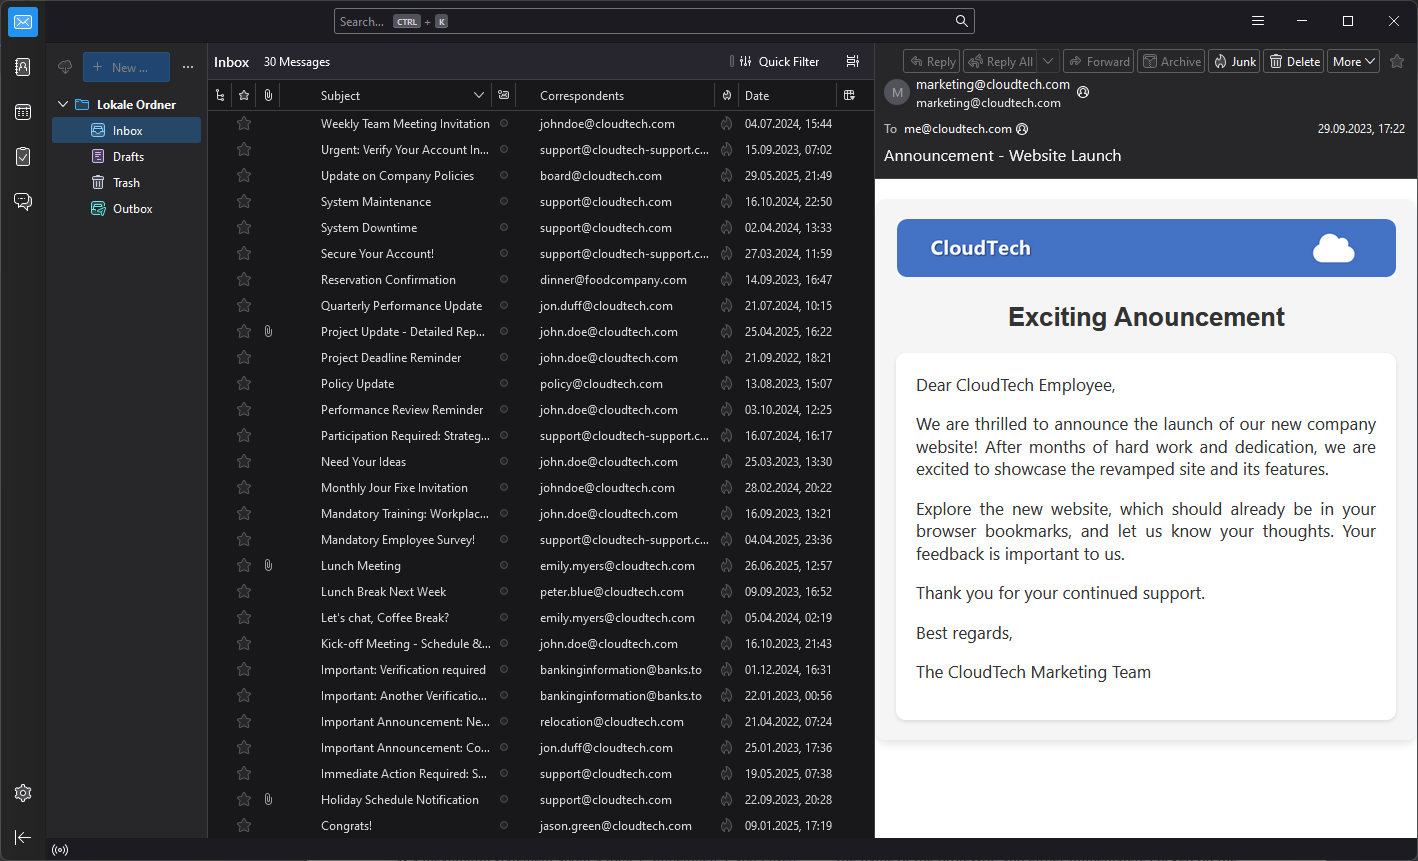
\includegraphics[width=0.8\linewidth]{figures/example2.png}
    \caption{Participants' environment in Mozilla Thunderbird.}
    \label{fig:example2}
\end{figure}

\begin{figure} [ht]
    \centering
    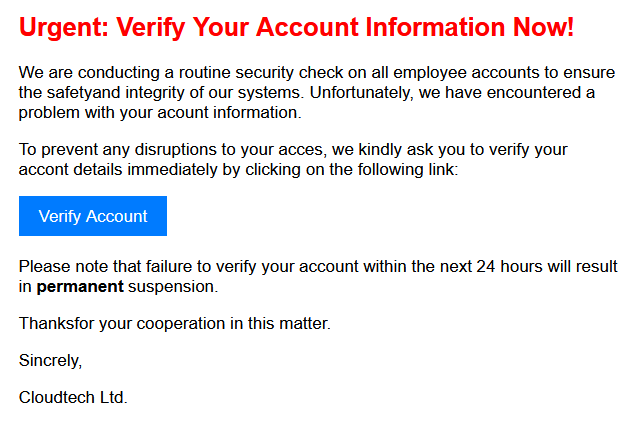
\includegraphics[width=0.6\linewidth]{figures/example.png}
    \caption{An example for a mock phishing email.}
    \label{fig:example}
\end{figure}

\section{Procedure}

\subsection{Consent, Demographics and ATI-S}

Before beginning with the study tasks, participants are required to sign a consent form that includes permissions for screen and audio recording as well as eye tracking. Following consent, they are asked to provide demographic information such as age, gender, educational background, and professional experience. Additionally, participants fill out the short version of the Affinity for Technology Interaction Scale (ATI-S)\footnote{https://ati-scale.org/}. This scale assesses individuals' comfort levels and predispositions towards technology, which helps to illuminate how these factors may influence their perceptions and interactions with phishing warnings. \newline
We opted to use the short version of the ATI scale due to its ability to efficiently measure technological affinity without imposing extensive questionnaire fatigue on participants and maintaining high engagement levels.

\subsection{Briefing and Setup}

Participants receive a briefing on the eye tracking process and a brief overview of Mozilla Thunderbird if they are not already familiar with its interface. The eye tracking calibration is conducted next to ensure accurate data capture. Audio recording is also enabled to capture the participants' verbal feedback throughout the study, facilitating later analysis of their qualitative responses. Participants are informed that they are welcome to ask questions at any time during the study to clarify any doubts or concerns they may have.

\subsection{Phase One: Sorting Task and Collection of Eyetracking Data}

Phase One serves as the quantitative backbone of our study, utilizing eye tracking technology to gather gaze data as participants engage with a series of emails. This phase is designed to simulate a real-world working environment to objectively assess how participants interact with our phishing warnings in a typical workflow. 

\textbf{Task Setup and Environment}

Participants are cast in the role of an employee at the fictional company "CloudTech". This setup is intended to create a realistic email environment. Upon commencement they are provided with a folder containing a mix of emails, including routine communications from fictional colleagues and company announcements. Within these emails there are several phishing attempts, though participants are not made aware of these inclusions to avoid biasing their responses.  

\textbf{Instructions and Procedure}

To simplify the email management task and ensure clarity, participants are instructed to discard any email into the trash folder that they suspect or deem unnecessary, without the need to further categorize or mark emails. This is designed to streamline the sorting process, allowing participants to focus more on the content and less on organizational tasks. 
During the sorting process, participants are encouraged to verbalize their thoughts and decisions. This "think aloud" method is crucial for understanding the decision-making process behind their actions.
\newpage
\textbf{Observer Role and Time Allocation}

The observer's role during this phase is to listen and monitor the explanations provided by the participants, intervening minimally (e.g. when questions arise) to avoid influencing their natural behavior. Each participant is allocated approximately 10 minutes to complete the task.

\subsection{Phase Two: Gathering Qualitative Feedback}

Following the sorting task, participants undergo a detailed semi-structured interview. They are asked about their subjective perceptions, their strategies for identifying phishing attempts and their opinions on the clarity and effectiveness of different warning designs.
This qualitative data enriches the study’s findings by adding personal personal context to the observed behaviours and eye tracking metrics. The interview questions cover several key areas:

\begin{itemize}
    \item General Perception: Inquiry into how participants perceived the warnings overall, including any elements that particularly stood out to them and the influence of the warnings on their decision making process.
    \item Effectiveness: Evaluation of the warnings' effectiveness presented during the study, identifying any warnings perceived as particularly helpful or less so. This includes a comparision between the different warnings.
    \item Design: Assessement of the warnings' design aspects, such as color, placement, and animations, and their impact on the users' attention.
    \item Personal Behaviour: Discussion around any new information noticed in the warnings that hadn't been considered before and typical behaviours when encountering phishing emails.
    \item Feedback: Suggestions for improving future iterations of the study and an opportunity for participants to raise any further questions or comments. 
\end{itemize}
 
The full study protocol and questioning framework is provided in appendix \ref{sec:protocol} and \ref{sec:interview}.

\begin{figure} [ht]
    \centering
    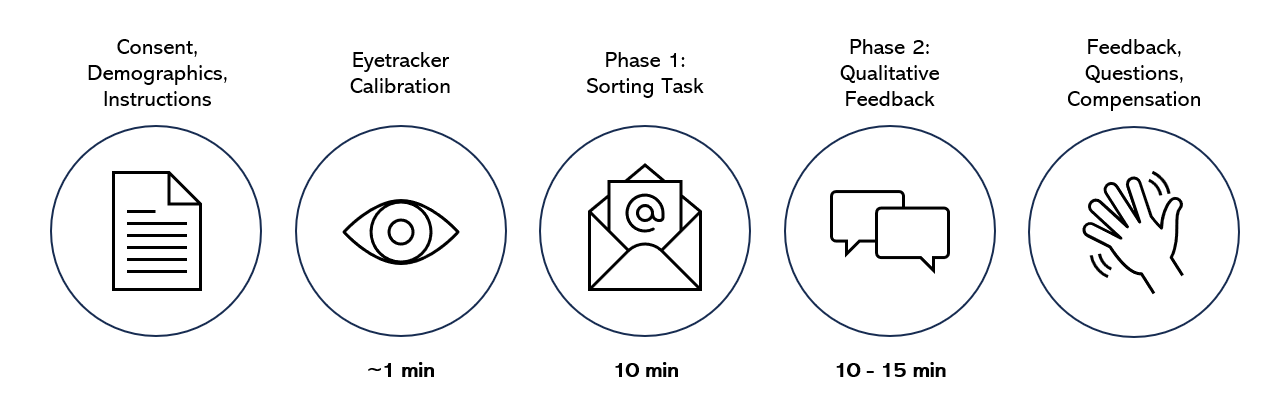
\includegraphics[width=1\linewidth]{figures/studysteps.png}
    \caption{Summary of the study procedure.}
    \label{fig:steps}
\end{figure}

\section{Data Analysis}
\subsection{Qualitative Data Analysis}
To enhance our understanding of participants' perceptions regarding different phishing warning designs, we employed a Qualitative Data Analysis (QDA) approach. Following established methodologies outlined in literature \cite{qda}, our method involved a hybrid coding strategy, combining both deductive and inductive techniques. Initially we established a set of codes based on our research questions and theoretical framework (deductive). As we analyzed the data, we expanded and refined this set to include new themes and patterns that emerged from participant feedback (inductive). This approach ensured that our analysis remained both structured and adaptive to the insights yielded by the study.

To facilitate this thorough and efficient exploration of qualitative data, we utilized MAXQDA2024. This software provided robust tools for organizing, coding, and analyzing the interview data, making the complex process of qualitative analysis more manageable and systematic. The project files are available in our GitHub repository, linked in appendix \ref{sec:github}.

Our coding framework captures the key dimensions of our research. Each main category and sub-category focuses on different aspects of how users interact with and perceive the visual and functional elements of phishing warnings. A detailed list of codes with explanations is provided in appendix \ref{sec:qda}. 

\begin{figure} [ht]
    \centering
    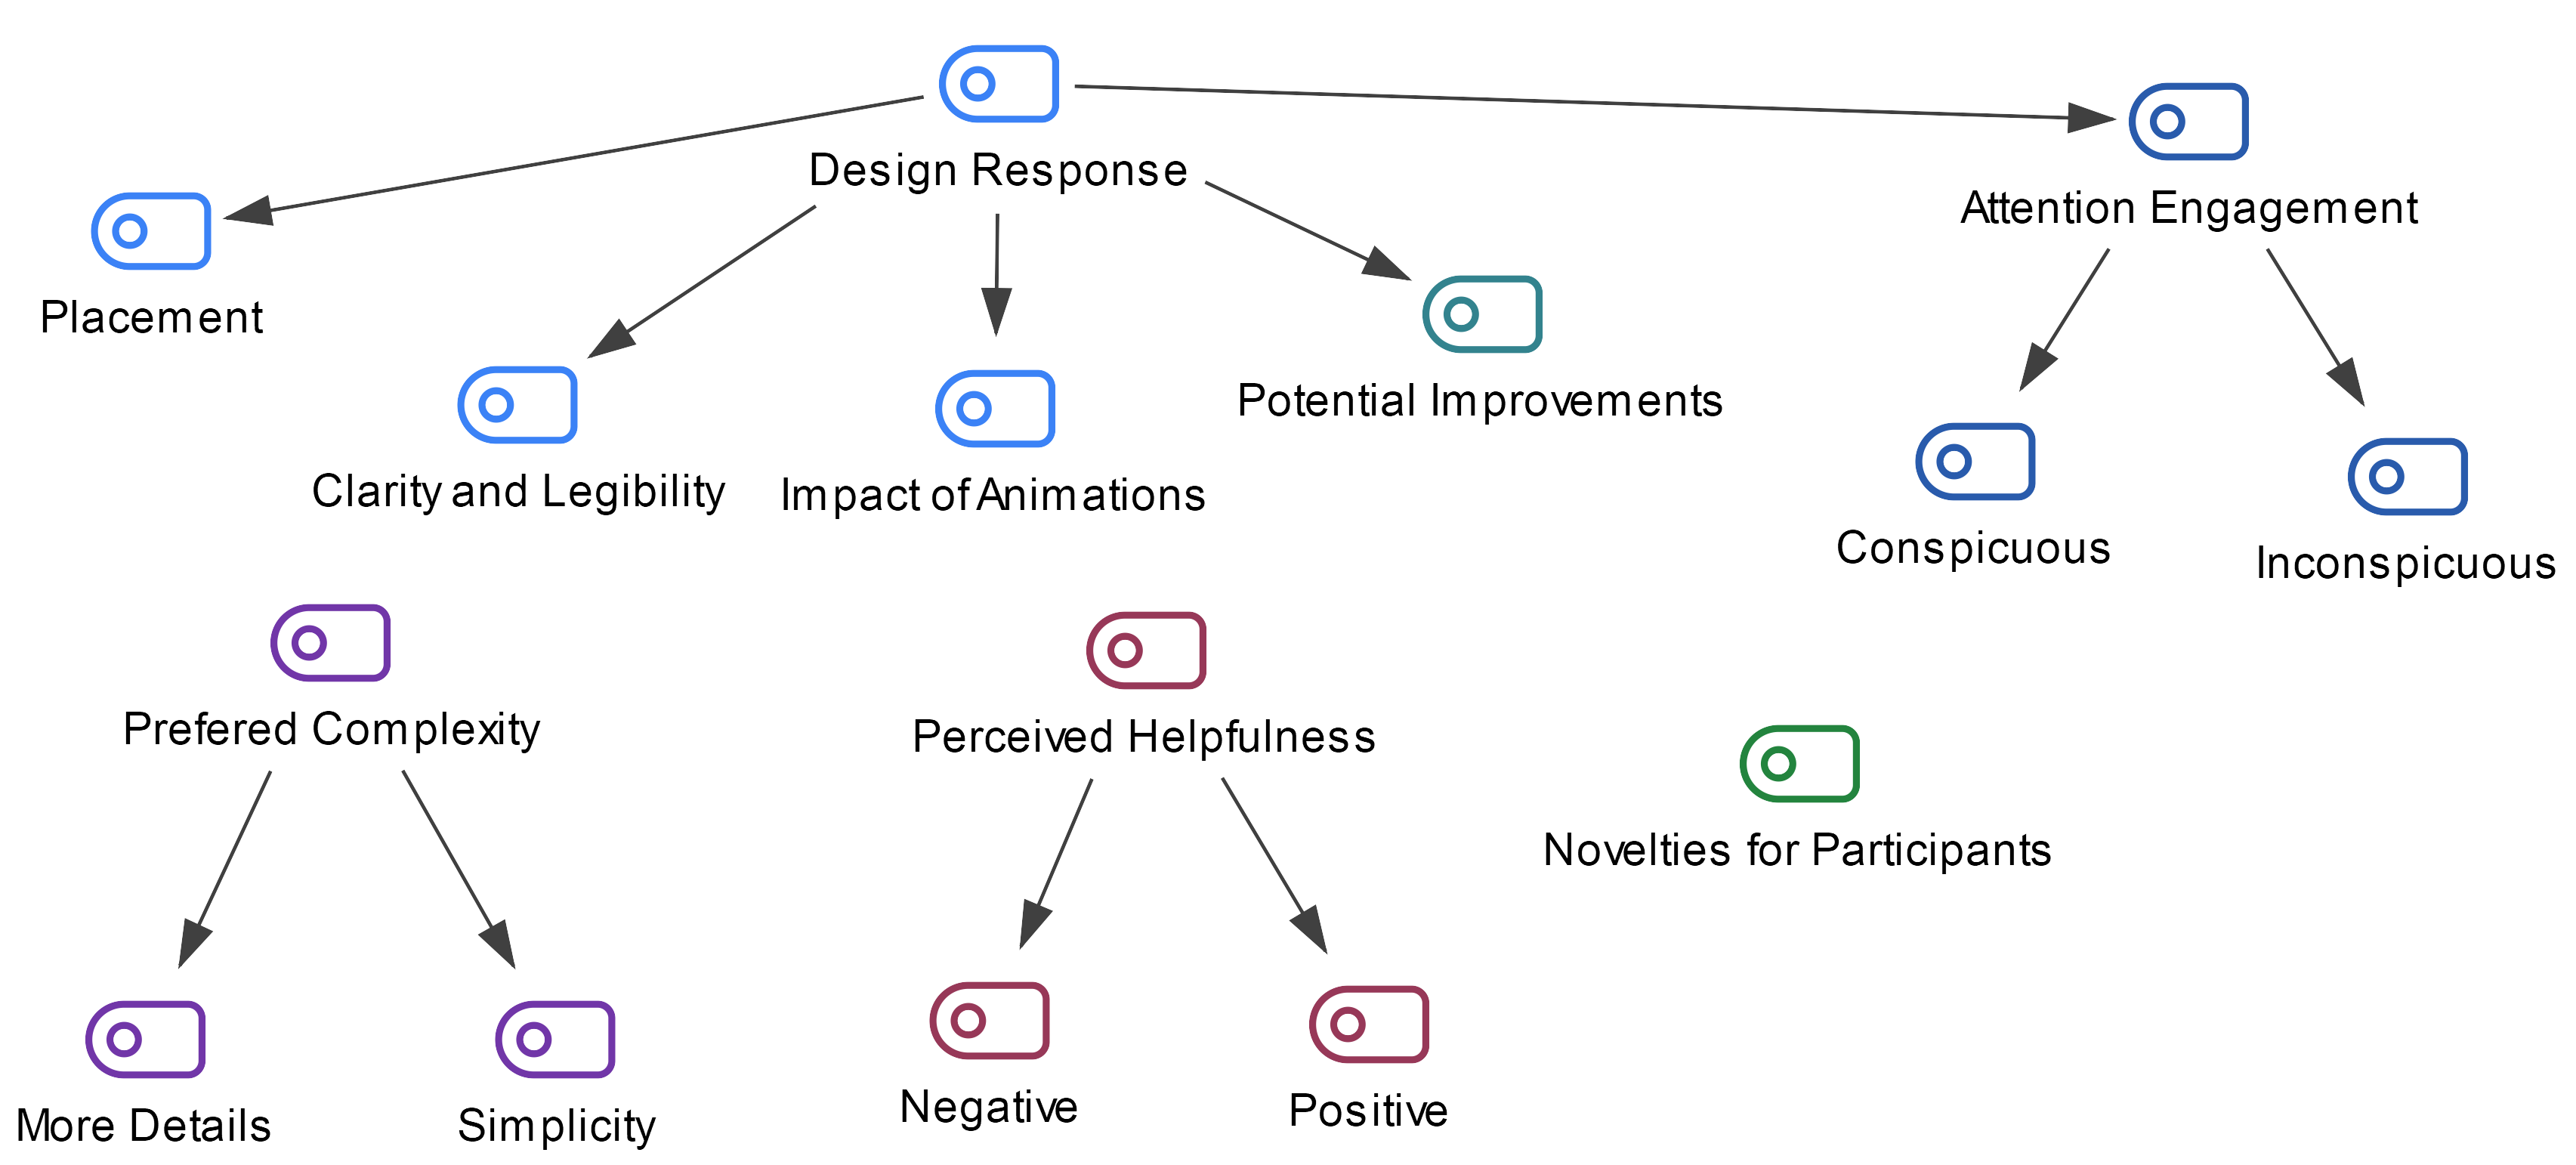
\includegraphics[width=0.9\linewidth]{figures/coding.png}
    \caption{Graphic illustration of our QDA codes, generated in MAXQDA 2024.}
    \label{fig:qda}
\end{figure}

\subsection{Eyetracking Data Analysis}
To evaluate the eye tracking data, we formulated the following hypotheses:

\begin{itemize}
    \item[\textbf{H1}] Delayed slide-in animations of warnings will disrupt typical email reading patterns and draw more attention.
    \item[\textbf{H2}] Warnings placed on the side of the email interface will be noticed later compared to those within the email body or at the top.
    \item[\textbf{H3}] Content integrated directly into the email body (e.g. Greeting or Signature Warning) will hold user attention for longer periods.
\end{itemize}

To analyze the eye tracking data, we used the Tobii Pro Lab software, which provided many tools for visualizing and interpreting gaze patterns. Our analysis involved several key tasks:

\begin{enumerate}
    \item \textbf{Defining Areas of Interest (AOI):} We defined specific AOIs within the email interface. This allowed us to quantify metrics such as fixation durations and frequencies for specific areas. The AOIs included different parts of the email where warnings were placed (see figure \ref{fig:aoi}).
    \item \textbf{Establishing Times of Interest (TOI):} To focus on critical moments of interaction, we defined TOIs. These were specific instances when participants opened emails containing warnings.
    \item \textbf{Visualization and Gaze Path Analysis:} Using Tobii Pro Lab’s visualization tools, we oberserved and analyzed gaze points. This was crucial for Hypothesis 1, as it allowed us to see how animations affected reading patterns.
\end{enumerate}

To align with our hypotheses, we collected the following eye tracking metrics:

\begin{enumerate}
    \item \textbf{Time to First Fixation:} This metric measures the time it takes for participants to fixate on a specific AOI after the email is presented \cite{eyetrack}. It helps us understand how quickly each warning design draws attention compared to others.
    \item \textbf{Average Fixation Duration:} By averaging the duration of all fixations within each AOI, we can assess the overall engagement level with different components of the email interface. Fixation durations range from 150-300ms, with higher durations meaning a higher level of engagement \cite{eyetrack}.
\end{enumerate}

These methods and metrics allowed us to test our hypotheses and evaluate the effectiveness of different phishing warning designs in capturing user attention.

\begin{figure} [ht]
    \centering
    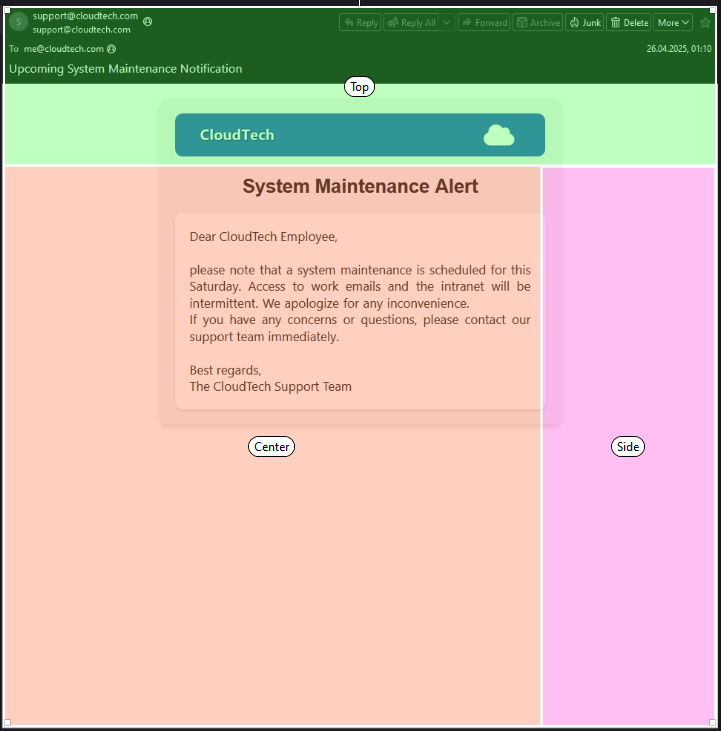
\includegraphics[width=0.7\linewidth]{figures/aoi.png}
    \caption{AOI zones in Tobii Pro Lab.}
    \label{fig:aoi}
\end{figure}

\chapter{Design and Implementation}
\label{implementation}

\section{Warning Types}
\label{types}
For our study we designed four primary types of phishing warnings, each having two different variations. These variations aim to explore different aspects of user interaction and attention.

\subsection{Group 1: General Alerts}

\textbf{Generic Banner:} A broad, non-specific warning that does not target any specific content within the email but serves as a general alert to the possibility of phishing.

\begin{itemize}
    \item Variant 1: The banner slides in from the top. This placement tests the immediate visibility and impact of warnings when users first open an email. 
    \item Variant 2: The banner is positioned on the right side of the email body. This alternative aims to assess how peripheral placement affects user noticeability and response compared to more traditional top placement.\par
\end{itemize}

\begin{figure} [h]
\centering
\begin{subfigure}{.5\textwidth}
  \centering
  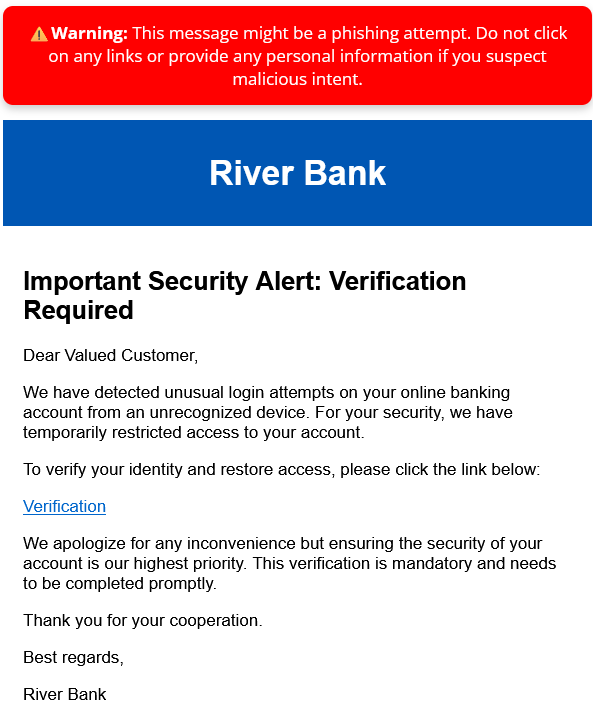
\includegraphics[width=.9\linewidth]{figures/banner1.png}
  \caption{Variant 1}
  \label{fig:banner1}
\end{subfigure}%
\begin{subfigure}{.5\textwidth}
  \centering
  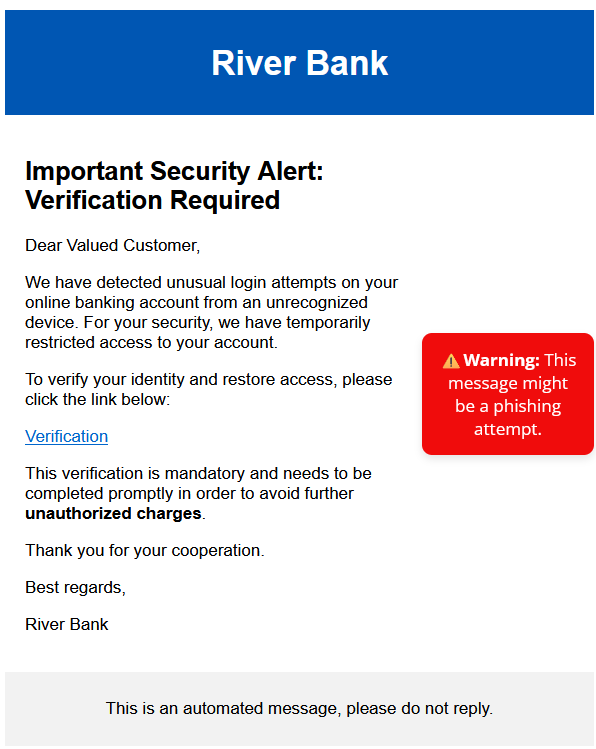
\includegraphics[width=.9\linewidth]{figures/banner2.png}
  \caption{Variant 2}
  \label{fig:banner2}
\end{subfigure}
\caption{Generic Banner}
\label{fig:banner}
\end{figure}
\newpage

\subsection{Group 2: Context-Aware Warnings}

\textbf{Tooltip Warning on Link Hover:} This warning appears when a user hovers over a link, providing immediate contextual information about the potential danger of the link, making it context-aware as it is specifically related to the actions the user is about to take (i.e., clicking a link). A tooltip appears, warning the user and preventing them from clicking the link. After a 3 second countdown, the tooltip moves to the side, making the link clickable at the users own risk. 

This approach aligns closely with the research conducted by Petelka et al. \cite{petelka}, which emphasizes the effectiveness of proximity and user interaction with link-focused phishing warnings in reducing susceptibility to phishing attacks. In this thesis, the tooltip warning activates when a user hovers over a link, immediately providing contextual information and temporarily blocking access to the link, thereby forcing the user to recognize and process the warning before proceeding. This method mirrors Petelka et al.'s findings that such forced interaction can significantly heighten user caution and awareness. Moreover, this study further explores the impact of varying levels of informational detail in the tooltips, assessing how these variations influence user perception.

\begin{itemize}
    \item Variant 1: Includes more detailed information within the banner, such as the actual URL. This version tests whether providing additional context within the warning influences user decisions about clicking on links.
    \item Variant 2: Presents less information, focusing on a simple cautionary message. The aim here is to evaluate the effectiveness of minimalistic warnings in deterring harmful interactions.
\end{itemize}

\begin{figure} [h]
\centering
\begin{subfigure}{.5\textwidth}
  \centering
  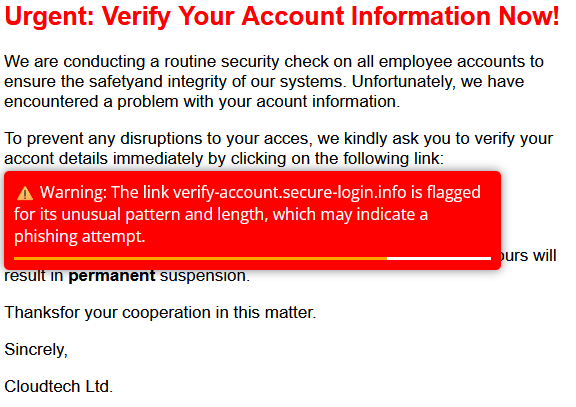
\includegraphics[width=.9\linewidth]{figures/hover1.png}
  \caption{Variant 1}
  \label{fig:tool1}
\end{subfigure}%
\begin{subfigure}{.5\textwidth}
  \centering
  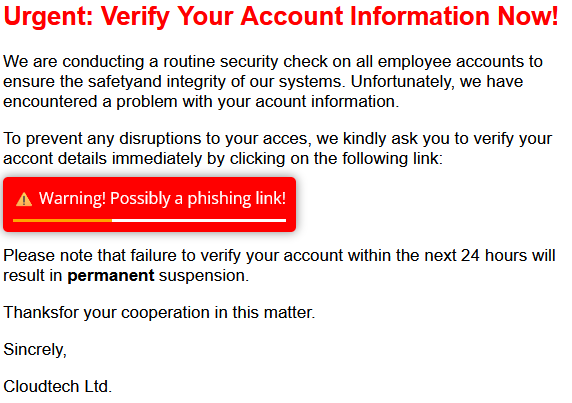
\includegraphics[width=.9\linewidth]{figures/hover2.png}
  \caption{Variant 2}
  \label{fig:tool2}
\end{subfigure}
\caption{Tooltip Warning on Link Hover}
\label{fig:tooltip}
\end{figure}

\subsection{Group 3: Content-Specific Warnings}

\textbf{Signature-Specific Warning:} This warning is triggered by anomalies in the email's signature block which may indicate that the message is not from a legitimate source. It focuses on deviations from standard or expected signature formats commonly seen in regular correspondence with the sender.

\begin{itemize}
    \item Variant 1: Accompanied by proof from past emails, offering a direct comparision to highlight discrepancies. This tests the baseline effectiveness of alerting users to potential signature anomalies with additional context.
    \item Variant 2: Presents less information, focusing on a simple cautionary message next to the signature. The aim here is to evaluate the effectiveness of minimalistic warnings in deterring harmful interactions.
\end{itemize}

\begin{figure} [H]
\centering
\begin{subfigure}{.5\textwidth}
  \centering
  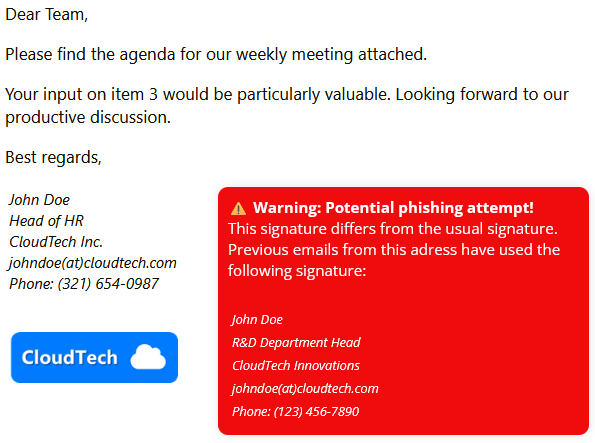
\includegraphics[width=.9\linewidth]{figures/signature1.png}
  \caption{Variant 1}
  \label{fig:sig1}
\end{subfigure}%
\begin{subfigure}{.5\textwidth}
  \centering
  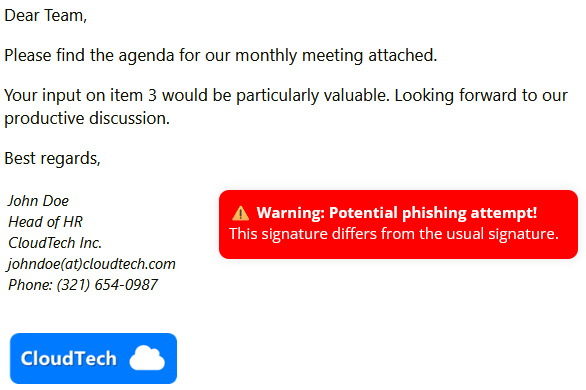
\includegraphics[width=.9\linewidth]{figures/signature2.png}
  \caption{Variant 2}
  \label{fig:sig2}
\end{subfigure}
\caption{Signature-Specific Warning}
\label{fig:signature}
\end{figure}

\textbf{Greeting-Specific Warning:}  Similar to the previously described signature warning, this alert focuses on irregularities in the email's greeting. It is designed to catch attention when the greeting does not match the usual formats, suggesting that the email could be a phishing attempt.

\begin{itemize}
    \item Variant 1:  Includes "proof" from past emails, similar to the signature warning variation. Additionally this warning banner is interactive, as the user can click on the corresponding email, opening it in a new tab. This is designed to see if direct comparisons with previous legitimate emails help users to better understand why the email might be a phishing attempt.
    \item Variant 2: Without additional context, focusing on a simple cautionary message next to the greeting. This variation assesses users' ability to detect phishing without the aid of explicit historical comparisons.
\end{itemize}

\begin{figure} [h]
\centering
\begin{subfigure}{.5\textwidth}
  \centering
  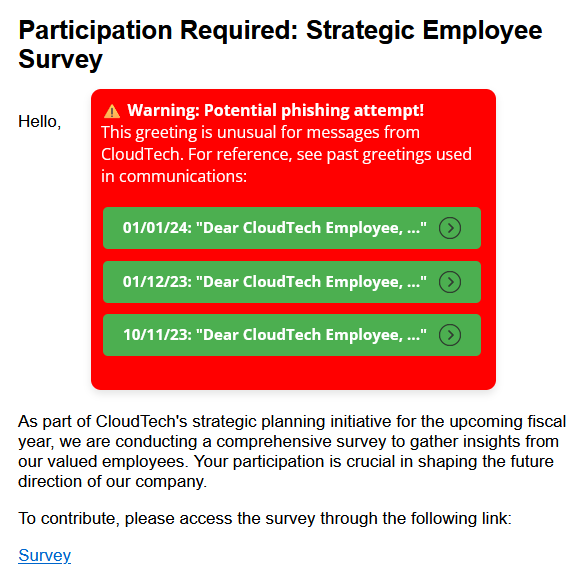
\includegraphics[width=.9\linewidth]{figures/greeting1.png}
  \caption{Variant 1}
  \label{fig:greeting1}
\end{subfigure}%
\begin{subfigure}{.5\textwidth}
  \centering
  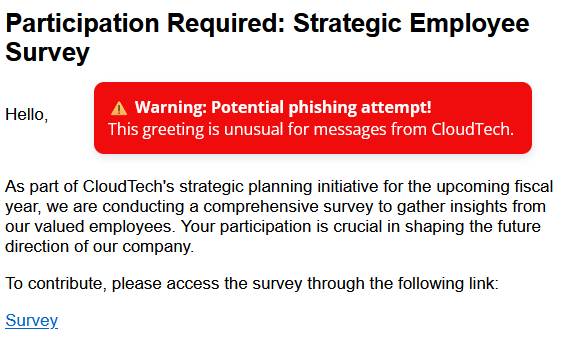
\includegraphics[width=.9\linewidth]{figures/greeting2.png}
  \caption{Variant 2}
  \label{fig:greeting2}
\end{subfigure}
\caption{Greeting-Specific Warning}
\label{fig:greeting}
\end{figure}

\section{Visual Design Strategy and Rationale}
We followed a visual design strategy for the phishing warnings developed in our study, aiming to merge aesthetics with functionality to create an effective warning mechanism. Building upon established research \cite{wogalter2002}, our design approach was crafted to enhance the salience, recognizability, and comprehensibility of warnings. We focused on several key elements identified in the literature as critical for maximizing the effectiveness of visual warnings: color usage, typography, and the inclusion of universally recognized symbols. These elements were chosen based on their proven ability to capture attention quickly and convey urgency effectively, ensuring that users could not only notice but also understand the warnings promptly and act accordingly.

\subsection{Color Scheme and Typography}
The choice of a vivid shade of red (hex: \#ff4d4d) for the background of our warnings leverages its psychological impact, as this decision is rooted in research indicating that red can trigger heightened alertness and caution \cite{kuniecki, wogalter2002}. The addition of a contrasting yellow triangle, serving as a pictorial symbol universally recognized for caution, further enhances the visibility and impact of the warnings. This use of universally understood symbols is supported by literature emphasizing the importance of immediate comprehension in warning design \cite{wogalter2002}. \newline
Rounded corners were introduced to the warning design to make the visual alerts appear more modern and less aggressive, maintaining user comfort without sacrificing visibility. This design choice aligns with contemporary design trends that favor user-friendly interfaces. \newline
The font choice, Segoe UI, was selected for its clarity and the decision to use bold fonts aims to further enhance readability.

\subsection{Animation and Timing}
Each warning features a sliding animation that initiates one second after the email is opened. This deliberate delay and the dynamic entrance of the warnings were designed to distinguish them clearly from the static email content. By introducing the warnings as distinct, dynamic elements, we aimed to disrupt the user's initial scan of the email content, drawing their focus directly to the alert and reinforcing the perception of the warnings as separate and urgent. Research supports this approach, showing that animations can significantly enhance the allocation of attentional resources, making such dynamic elements more effective at capturing and holding viewer attention \cite{muller}. This strategic use of animations is therefore critical in ensuring that the warnings are not only noticed but also perceived as immediate and pressing alerts.

\section{Iterative Design Adjustments}
\label{adjust}
Over the course of the study, feedback from participants highlighted several areas for improvement in our warning designs. This led to an iterative design process, where modifications were made to enhance clarity and legibility. The new warnings were implemented from the twelfth participant onwards. This allowed us to compare the effectiveness of the original and modified designs directly within the same study framework. Here are the key adjustments made:

\begin{itemize}
    \item \textbf{Color and Typography:} We intensified the shade of red used for the warning backgrounds to a deeper, more vivid tone (hex: \#f00c0c). The font was changed to 'Open Sans' and we also used more bold fonts. This resulted in a generally more legibile design.
    \item \textbf{Animation Timing:} We removed the delay in the animations, allowing warnings to appear immediately as the email is accessed.
    \item \textbf{Greeting-Specific Warning:} 
    The buttons that link to previous emails for comparison have been updated to more clearly indicate that they are interactive.
\end{itemize}

The figures in section \ref{types} already incorporate these changes. An overview of our first iteration of the warning types is provided in appendix \ref{sec:warnings}.

\section{Technical Background}
\subsection{Email Client}
Our experimental setup was anchored in Mozilla Thunderbird, selected for its adaptability in customizing email functions via plugins. We utilized a portable installation of Thunderbird\footnote{\href{https://www.thunderbird-mail.de/lexicon/entry/44-portable-thunderbird/?l=2}{https://www.thunderbird-mail.de/lexicon/entry/44-portable-thunderbird/?l=2}}, which facilitated an easy setup and ensured portability between setups. Custom emails were directly placed into the local folder of Thunderbird, eliminating the need for participants to log into an actual email account, thereby simplifying the process and enhancing security. This approach also simplified the process of resetting the setup after each participant, ensuring consistency and efficiency across sessions.

\subsection{Emails and Custom Plugin}
To faciliate the integration of phishing warnings into the emails, the warnings were directly embedded into the HTML structure of each email. This integration was aimed at replicating how an email client's security system might naturally react to detecting potential threats.\newline
Additionally, a custom plugin was developed to enhance the functionality of the phishing warnings embedded within the email content. Utilizing Mozilla Thunderbird's WebExtensions API\footnote{ \href{https://webextension-api.thunderbird.net/}{https://webextension-api.thunderbird.net/}} and JavaScript code, this plugin was engineered to introduce dynamic visual cues, such as animations and interactive elements.
The core functionality of the plugin centers around its capability to inject JavaScript code directly into the HTML of each email. This injection process is crucial as it allows for real-time modification of the email content, thereby enabling animations that draw the user's attention to specific areas of concern and interactive features that provide additional context.

\textbf{Check Email Subject}

As we only want our warnings to appear for a predefined set of emails, the plugin first checks the subject line of the email that is currently viewed. If it detects one of our predefined phishing emails, the plugin dynamically injects the necessary scripts into the email's HTML content. This method ensures that the interactive warnings and animations are only activated when relevant. 

\textbf{Event Listeners}

For our hover-triggered tooltips on suspicious links we added an event listener to the hyperlink, which listens for mouse events and triggers the appearance of the tooltip when necessary. \newpage

\textbf{Animations}

For animations we used the CSS @keyframes at-rule\footnote{ \href{https://developer.mozilla.org/en-US/docs/Web/CSS/@keyframes}{https://developer.mozilla.org/en-US/docs/Web/CSS/@keyframes}}. Doing this via the plugin was strictly necessary as Mozilla Thunderbird does not natively support animations embedded in the HTML code of emails. 

\textbf{Interactive Elements}

This plugin also makes the functionality of variant 1 of our greeting-specific warning (\ref{fig:greeting1}) possible. Within the HTML of the email, we embedded a list that represents past emails. The plugin expands each list item with an interactive capability: clicking any list entry opens a new tab displaying the content of the corresponding past email. Additionally the plugin handles the styling of the buttons. It applies a green background color to indicate interactivity and sets the cursor to a pointer, visually cueing users that the entries are clickable. 

\textbf{Mock Phishing Page}

We implemented a feature in the plugin to handle cases when users click on links within our mock phishing emails. Upon doing so, our plugin redirects them to a mock phishing page, designed to simulate the potential consequences of clicking on a phishing link. In terms of the technical implementation, the feature operates by attaching an event listener to each hyperlink within the mock phishing emails. When a link is clicked, rather than following the original URL, the event listener intercepts this action and instead directs the user to our predefined HTML page. This workaround was necessary as Mozilla Thunderbird restricts plugins from directly embedding links in emails for security purposes.

\begin{figure} [ht]
    \centering
    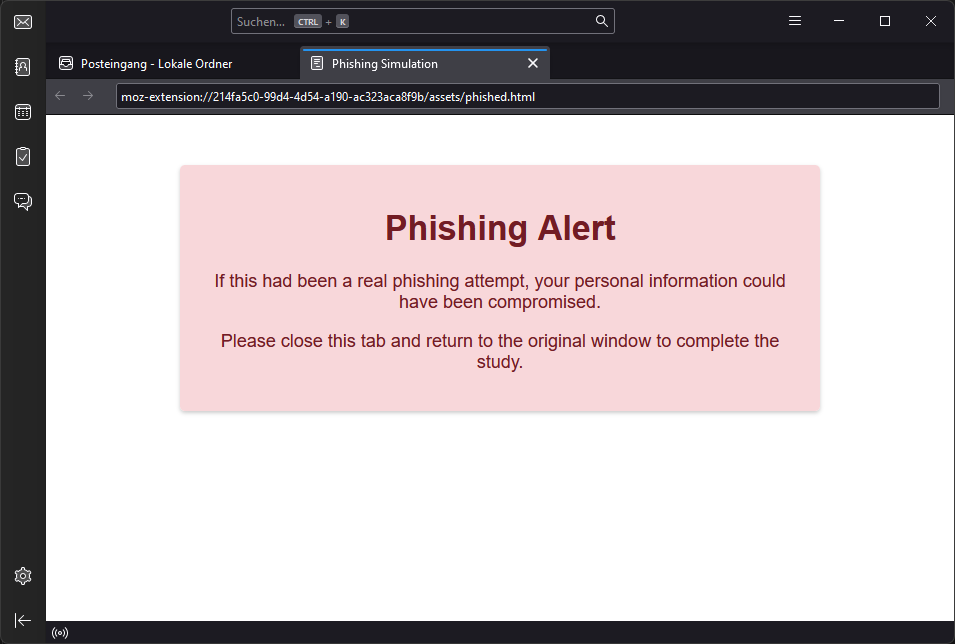
\includegraphics[width=1\linewidth]{figures/mockpage.png}
    \caption{Mock phishing page when participants click on links.}
    \label{fig:mock}
\end{figure}


\subsection{Python Script to Shuffle Emails}
Additionally, a Python script was utilized to shuffle the date of each email. As the emails were sorted by their corresponding dates, this allowed us to randomize the order of the emails for each participant. This step was critical to minimize any sequence bias and ensure that each participant's exposure to the emails was unique, thereby providing a more robust measure of the warnings' effectiveness across varied contexts. The full source code of the plugin, the Python script, and the emails, will be provided in appendix \ref{sec:github}, accessible through a GitHub repository.

\chapter{Results}
\label{results}

\section{Questionnaire Data}
\subsection{Demographics}
\begin{table}[ht]
\centering
\begin{tabularx}{\textwidth}{Xcc}
\toprule
\textbf{Demographics} & \textbf{Total (N=16)} & \textbf{\%} \\
\midrule
\textbf{Age} \\
\quad 20 - 29 & 13 & 81.25 \\
\quad 30 - 39 & 2 & 12.50 \\
\quad 40+ & 1 & 6.25 \\
\midrule
\textbf{Gender} \\
\quad Male & 10 & 62.50 \\
\quad Female & 6 & 37.50 \\
\quad Non-binary & 0 & 0.00 \\
\quad Prefer not to tell & 0 & 0.00 \\
\midrule
\textbf{Education} \\
\quad Doctorate degree & 1 & 6.25 \\
\quad Graduate degree & 2 & 12.50 \\
\quad Undergraduate degree & 9 & 56.25 \\
\quad High school diploma & 4 & 25.00 \\
\quad Secondary education & 0 & 0.00 \\
\quad Other & 0 & 0.0 \\
\midrule
\textbf{Profession} \\
\quad Student & 13 & 87.5 \\
\quad Research Assistant & 1 & 6.25 \\
\quad Retiree & 1 & 6.25 \\
\bottomrule
\end{tabularx}
\caption{Demographic data collected in the survey.}
\end{table}

The demographic data from our study primarily shows a young participant base with 81.25\% aged between 20-29, primarily students (87.5\%). The gender distribution was majority male (62.50\%) with the remainder female. Most participants had at least some university education, with 56.25\% holding an undergraduate degree and a smaller number having graduate degrees or a high school diploma. This generally younger demographic was anticipated, as the recruitment strategies employed were focused on platforms commonly frequented by younger audiences, such as university chat groups on Discord, WhatsApp, and Slack, as well as through the LMU newsletter.

\subsection{ATI-S Scale}

\begin{figure}[H]
\centering
\begin{tikzpicture}
    \begin{axis}[
        ybar,
        symbolic x coords={Very Low, Low, Medium, High, Very High},
        xtick=data,
        nodes near coords,
        nodes near coords align={vertical},
        ymin=0,ymax=16,
        ylabel={Number of Participants},
        xlabel={Affinity Levels},
        %title={ATI-S Scale (Affinity for Technology Interaction)}
    ]
    \addplot coordinates {(Very Low,0) (Low,1) (Medium,3) (High,11) (Very High,1)};
    \end{axis}
\end{tikzpicture}
\caption{Distribution of Affinity for Technology Interaction among participants.}
\label{ati}
\end{figure}

A significant aspect of the participant profile is their technological affinity, as indicated by the Affinity for Technology Interaction Short Scale (ATI-S) values. This data revealed a pronounced tendency towards technology, with 12 participants scoring high or very high in technology affinity. This implies that the majority of participants were not only familiar with but also comfortable using technology, which is a crucial consideration in the context of phishing awareness and the effectiveness of warnings.

\section{Interview Results}

\textbf{Design Response}

Clarity and Legibility: Participants generally found the color red effective in drawing attention, with one noting \textit{"The red is just very catchy"} (P9), highlighting the visual impact of vibrant colors. The legibility of warnings was often a concern, as evidenced by comments such as \textit{"It’s the white on red what makes it difficult to read at times."} (P9), indicating difficulties with text contrast. 

Impact of Animations: Animations were noted for their effective attention-grabbing capabilities. For instance, one participant mentioned, \textit{"When the text field moves in like this, your eyes automatically move there."} (P2), showing how animations guide viewers' focus. A participant remarked on the possible negative impact of frequent animations, stating, \textit{"Moving warnings are more noticeable than ones that just appear on the screen. But if you put moving warnings on all phishing mails, it might be overwhelming and tire the eyes and mind. A balance is necessary. Maybe being too flashy, could even lead to desensitization over time."} (P5) Some participants also noted that the animations were too slow to appear, \textit{"It would be better if the warnings appeared immediately upon opening the email instead of having a delay"} (P5), which could lead to critical oversights. 
    
Placement: Participants commonly observed that warnings placed on the side of the email were less noticeable, often residing in their peripheral vision. As one participant expressed, \textit{"I actually found this one a bit inconspicuous because you have the email body here and the warning there. It reminds me of those advertisements on websites placed on the side of the page."} (P1) Conversely, warnings integrated directly into the email body proved to be more conspicuous. Participants reported that these warnings grabbed their attention immediately upon opening the email, as they were in the direct line of sight while reading the email content. 


\textbf{Perceived Helpfulness}

Context-Aware Warnings (Tooltip on Hover Over Link): This type of warning was generally seen as highly effective because it actively prevents clicks on potentially malicious links. A participant mentioned, \textit{"I believe the one covering the link was the most effective because it immediately prevented interaction."} (P6).
    
Content-Specific Warnings (Signature and Greeting Warnings): This type of warning was appreciated for its specificity, noting that these kind of details are easily overlooked in phishing emails: \textit{"I really liked the signature warnings. That could be something that might not catch the user’s attention at all."} (P5). A common point of criticism was, that this kind of warning is often not applicable, as not every email, especially in a non-business context, ends with a signature or uses a consistent greeting.
      
General Alerts: This type of warning received mixed feedback due to their positioning and the lack of detailed information they provided. Participants noted its visibility issues and expressed a preference for warnings that include explanatory details about the alert: \textit{"Those that just flew in and had standard text might be the weakest."} (P6). 

\textbf{Preferred Level of Detail}

A key theme that emerged from the interviews was a clear division in preference for either more detailed warnings or simpler alerts. Participants who favored more details appreciated the additional context and explanations provided in the warnings, which helped them understand why an email was flagged as suspicious. One participant stated, \textit{"I preferred the longer ones, because it teaches me how to recognize future phishing attempts."} (P11), emphasizing the educational aspect. Another point mentioned was the fact that a longer explanation might make it easier and more helpful for non tech-savy people. The Greeting Warning with interactive buttons presented a unique challenge during the study. While intended to enhance user engagement by providing direct context and proof, many participants either did not realize the buttons were clickable or hesitated to use them. This hesitation stemmed from a fear that interacting with the buttons might inadvertently lead them into a phishing trap. One participant expressed, \textit{"I wouldn’t like to click on those buttons if I would get such a warning. I don’t really know if I can trust it."} (P16). \par
Conversely, some participants (P5, P6) preferred simple warnings, valuing the straightforwardness and immediacy of the message without additional information. This preference indicates that for some users, efficiency and speed in email processing are prioritized over detailed educational content. 

\textbf{Novelties for Participants}

The qualitative data analysis underscored that many participants found the greeting and signature-specific warnings to be novel features. These aspects of the phishing warnings introduced new elements that participants had not previously encountered or considered significant in identifying phishing emails. As one participant reflected, \textit{"I have not seen such tailored warnings in phishing emails, which recognize a specific pattern and tell you why it's a phishing attempt. That is very new to me."} (P13). \newpage

\textbf{Refining Warning Design: Incorporating Feedback}

As outlined in section \ref{adjust}, modifications were made to the phishing warning designs beginning with participant 12. 
These changes were positively received, as indicated by subsequent participant feedback. Post-adjustment, there were no further complaints regarding the readability of the text or the timing of the animations, except for a single comment about the red tone being potentially too strong (P15). Participants appreciated the quicker responsiveness and greater clarity of the warnings, which effectively addressed the initial concerns raised about legibility and the timing of animation effects. 

\section{Eye Tracking Results}
\label{sec:eyetrackingres}
During the data analysis phase, it was noted that the eye tracking data for one participant (P14) was significantly lower in sample size compared to others. This anomaly could be attributed to improper seating position or a flawed calibration process. To maintain the integrity and reliability of the analysis, this participant's data was excluded, resulting in a total of 15 eye tracking samples being considered for the final evaluation.

A full export of our raw eyetracking data is provided in the GitHub repository linked in appendix \ref{sec:github}.


\textbf{H1: Delayed Animation's Influence on Reading Pattern}

Eye tracking data indicated no significant disruption in reading patterns due to delayed animations in phishing warnings. Observing the gaze patterns showed that the onset timing of animations, whether immediate or delayed, did not alter the attention flow significantly. Users exhibited similar engagement with immediate and delayed warning presentations, suggesting a uniform approach to processing these visual cues.

\textbf{H2: Visibility of Side-Placed Warnings} 

The eye tracking analysis showed that warnings positioned on the side of the email interface captured attention quickly but consistently later than other warnings. The focus of gaze primarily remained on the other areas of the emails, with peripheral warnings drawing attention only after the central and top content had been reviewed. This observation was consistent across the study's participants, supporting the hypothesis that side-placed warnings are less immediately noticeable. \newline Eye tracking data (figure \ref{sideaoi}) supports this finding, showing that the median time taken for participants to first fixate on the Side AOI was approximately 2 seconds. To put this in contrast we compared this to the Top AOI data, where we recorded a notably quicker median time to first fixation of approximately 1.2 seconds.  

\textbf{H3: Sustained Engagement of Body-Integrated Warnings}

Data strongly supported the hypothesis that warnings integrated directly into the email body were engaged with more thoroughly by users than those placed at the side. The analysis of average fixation durations (figure \ref{avgfix}) revealed that engagement times for the Center AOI were generally longer across participants. However, there were notable exceptions for participants 7 and 13, where the fixation duration on the Center AOI was shorter compared to the other participants. 

\begin{figure}[H]
\centering
\begin{tikzpicture}
\begin{axis}[
    xlabel={Participant ID},
    ylabel={Time to First Fixation (seconds)},
    grid=major,
    xmin=0, xmax=16, 
    ymin=0, ymax=15,  
    xtick={1,2,...,15}, 
    xticklabels={1,2,...,12,13,15,16}, 
    xticklabel style={font=\footnotesize, rotate=0}, 
    yticklabel style={font=\footnotesize}
]
\addplot+[
    only marks,
    mark=*,
    mark size=2.5pt,
    scatter=true, 
    color=blue, 
    fill=blue  
] table [row sep=\\,y=data, x=seq] {
    seq  data\\
    1    1.95\\ 2    10.17\\ 3    1.46\\ 4    14.01\\ 5    2.32\\
    6    0.99\\ 7    1.58\\ 8    2.21\\ 9    1.91\\ 10   3.59\\
    11   1.91\\ 12   7.79\\ 13   1.37\\ 14   1.18\\ 15   1.31\\
};
\end{axis}
\end{tikzpicture}
\caption{Time to first fixation for the side AOI.}
\label{sideaoi}
\end{figure}

\begin{figure}[H]
\centering
\begin{tikzpicture}
\begin{axis}[
    xlabel={Participant ID},
    ylabel={Average Fixation Duration (milliseconds)},
    grid=major,
    xmin=0, xmax=16, 
    ymin=0, ymax=500,
    xtick={1,2,...,15}, 
    xticklabels={1,2,...,12,13,15,16}, 
    ytick={0, 100,200,300,400,500}, 
    xticklabel style={font=\footnotesize}, 
    yticklabel style={font=\footnotesize},
    legend style={
        at={(0.1855,0.83)},
        anchor=south,
        text width=2cm, 
        minimum width=2.5cm, 
        font=\footnotesize 
    }
]
\addplot+[
    scatter,
    only marks,
    mark=*,
    mark size=2.5pt,
    scatter=false,
    color=blue, 
    fill=blue 
] coordinates {
    (1,290) (2,270) (3,290) (4,270) (5,370)
    (6,270) (7,220) (8,280) (9,250) (10,300)
    (11,260) (12,470) (13,210) (14,240) (15,260)
};
\addplot+[
    scatter,
    only marks,
    mark=square*,
    mark size=2.5pt,
    scatter=false,
    color=red, 
    fill=red
] coordinates {
    (1,210) (2,170) (3,200) (4,210) (5,150)
    (6,180) (7,340) (8,160) (9,160) (10,120)
    (11,230) (12,190) (13,300) (14,200) (15,200)
};
\legend{Center AOI,Side AOI}
\end{axis}
\end{tikzpicture}
\caption{Comparison of the average fixation duration for center and side AOIs.}
\label{avgfix}
\end{figure}

\chapter{Discussion}
\section{Interpretation of Qualitative Feedback}
\subsection{Emerging Themes and Best Practices}
The qualitative feedback analysis illuminates several emerging themes that contribute to the effectiveness of phishing warnings. Reflecting on these, we can delineate best practices for designing phishing warning systems that align with user expectations.

\textbf{Attention-Grabbing without being Overwhelming}

A recurring theme is the delicate balance between capturing users’ attention and avoiding sensory overload. Warnings that are too subtle may go unnoticed, while those that are too aggressive could be dismissed as annoyances. Best practices suggest employing moderate animations and placing warnings within the users' immediate visual field. For example, one participant noted, \textit{"When the text field moves in like this, your eyes automatically move there."} (P2) indicating the value of animated cues. However, animations should not be excessively flashy or complex, as they risk desensitizing users over time. Supporting this, a study on the effects of animation in online contexts found that while animations increase visibility and engagement, they must be balanced to avoid overshadowing important content or overwhelming the viewer \cite{cheung}.

\textbf{Clarity and Contextual Information}

Clarity in warning messages is essential. Participants expressed a preference for warnings with a clear and legible typography set against a contrasting background, improving readability. The use of the color red was frequently mentioned as effective due to its association with caution and urgency. \newline 
Moreover, providing contextual information within the warning, such as the reason an email was flagged and highlighting subtle language cues, such as the greeting, can enhance users’ understanding and prompt more informed action. As one user aptly put it, \textit{"I preferred the longer ones, because it teaches me how to recognize phishing attempts."} (P11), highlighting the educative function. \newline
This emphasis on context-rich warnings aligns with findings from other studies \cite{buono, aneke}, which also highlight the importance of explanatory warnings in phishing emails, thus not only alerting users to immediate threats but also equipping them with knowledge that could prevent future phishing attacks. Such strategies are crucial for improving user understanding and ensuring that warnings lead to informed actions and thereby enhancing the overall effectiveness of phishing warnings.

\textbf{Trust and Interactivity}

The trustworthiness of warnings is key; users must feel confident interacting with them. This includes a hesitance to engage with clickable elements within the warnings due to fear of intensifying a potential threat. Best practices would therefore involve clearly distinguishing warning elements from potential phishing mechanisms and ensuring that interactive components, when used, are immediately recognizable as safe and official parts of the email client interface.

\textbf{Incorporating User Feedback for Iterative Improvement}

The inclusion of user feedback into the design process is not only beneficial but essential for the development of effective phishing warnings. Adjustments made in response to participant insights, such as enhancing color contrast to improve legibility, exemplify how iterative design based on user experience can significantly help in designing effective security measures. As highlighted in the article by Grobler et al. \cite{grobler} actively engaging users in refining security solutions helps tailor these systems to better meet their needs and expectations, thereby increasing their efficacy and user adoption rates. Best practices would therefore advocate for continuous user testing and refinement, ensuring that warnings adapt over time to align with evolving user behaviors and phishing tactics. This proactive approach ensures that security measures remain robust, user-friendly, and effective in real-world scenarios.

\subsection{Summary: Users’ Perceptions of Phishing Warnings}
To address RQ1 regarding user perceptions and the effectiveness of various phishing warnings in email interfaces, we analyzed qualitative feedback from participants. The effectiveness was assessed based on the ability of warnings to enhance user awareness, encourage appropriate actions to mitigate risks, such as not clicking on malicious links, and improve recognition of phishing threats in future encounters.

\textbf{Perceived Helpfulness and Effectiveness of Warning Types}
\begin{enumerate}
    \item \textbf{Context-Aware Warnings (Tooltip on Hover Over Link):}
    Participants found context-aware warnings extremely effective. These warnings prevent direct interaction with malicious links, thereby immediately mitigating risk. This direct intervention makes them highly valuable in protecting users in real-time.
    \item \textbf{Content-Specific Warnings (Signature and Greeting Warnings):}
    These warnings are appreciated for their specificity and relevance, particularly in environments where consistency is expected, such as professional emails. They provide clear and relevant context by highlighting anomalies in expected email patterns, offering a direct comparison with typical content. Their educational value is significant as they enhance users' ability to identify subtle signs of phishing attempts, which might otherwise be overlooked.
    \item \textbf{Generic Banners:}
    Generic banners received the least favorable feedback. Their effectiveness was often questioned due to poor placement and lack of detailed information, which led to them being easily ignored. Especially variant 2 (side placed banner) was criticized for being too inconsipicous. Participants compared its noticeability to peripheral advertisements on websites, which are often disregarded due to desensitization. This feedback highlights the importance of not only the placement of warning banners but also the inclusion of specific reasons why an email might be flagged as potentially dangerous, enhancing user understanding and response to phishing threats.
\end{enumerate}

\textbf{Preferred Warning Design}

From the feedback, it's clear that users prefer warnings that are not only visible but also informative. Warnings that blend seamlessly into the user's workflow in the email interface, such as those integrated within the primary content, are particularly effective. These warnings grab attention quickly, provide essential information, and are directly interacted with, enhancing both immediate and long-term phishing threat recognition.

\definecolor{Ebb}{rgb}{0.925,0.894,0.894}
\begin{table} [H]
\centering
\begin{tblr}{
  row{1} = {Ebb},
  hlines,
  vlines,
  hline{1,5} = {-}{0.08em},
  colspec = {X[1.75,l] X[2.25,l] X[4,l]},
}
\textbf{Warning Type}     & \textbf{Key Feature}                 & \textbf{User Feedback}                                                                                                      \\
Context-Aware       & Actively prevents clicking on links  & Very positive; users felt it was very effective and helpful, appreciating the proactive nature of the warning.              \\
Content-Specific    & Highlights anomalies in the language & Positive; users appreciated their specificity and educational value, noting they felt more informed about phishing tactics. \\
General             & Broad, non-specific warning          & Less favorable; often overlooked, reported by users as too generic and lacking actionable details.                          
\end{tblr}
\caption{Overview of warning types and user feedback.}
\label{tab:types}
\end{table}

\section{Interpretation of Eye Tracking Results}

\subsection{Impact of Delayed Animations}

Our hypothesis that delayed animations would disrupt the typical email reading pattern and draw more attention was not supported by the data. The implications suggest that while animations serve as useful attention-grabbing tools, their effectiveness does not necessarily benefit from a delayed presentation. Aligning with the qualitative interview results, it appears that ensuring the visibility of warnings immediately upon email viewing is more crucial for capturing attention and facilitating prompt user reactions. \newline
However, it is important to note, that the evaluation of this hypothesis may be limited by the methodology used. Only 4 participants tested the new warnings with no animation delay, which may not provide a sufficiently robust dataset to draw definitive conclusions.

\subsection{Effective Warning Placement}

The data strongly supports that warnings placed within the central viewing area of an email are engaged with more extensively. This is evidenced by generally longer average fixation durations on the Center AOI. These findings underscore the efficacy of aligning warning placements with natural reading behaviors, thereby enhancing the visibility and impact of security warnings. \newline However, the analysis revealed notable deviations for participants 7 and 13, who exhibited shorter fixation durations on the Center AOI compared to other participants. This variability in user interaction suggests that while centrally-placed warnings are generally effective, their impact can vary significantly among users due to individual differences in reading habits or the visual salience of the warnings. \newline
The extended engagement with central warnings highlights their effectiveness in maintaining user attention, which is crucial for ensuring that warnings are not only noticed but also sufficiently processed. This is vital for the effective communication of security-related information. Based on these insights, designers are encouraged to position crucial information and alerts within the central visual field to maximize their impact. Furthermore, understanding the reasons behind the shorter fixation times for specific participants could inform more tailored design approaches, ensuring that warnings are effective across a diverse user base.

In contrast, warnings positioned on the periphery of the email interface, such as on the sides, were consistently noticed later and engaged with less extensively. Although our data indicates only a slight delay in detection, this brief period can be critical, particularly during a hectic workday when users may be under pressure or multitasking. This oversight provides a window during which users could inadvertently interact with deceptive links or other malicious content. Moreover, the presence of outliers where the time to first fixation was exceedingly long highlights the potential severity of this issue. \newline
Furthermore, the average fixation duration on these side-placed warnings was also notably lower than that for central warnings, suggesting that even when the warning is noticed, the engagement is less intensive. This lack of deep engagement suggests that the warnings may not be registering effectively with users. This observation aligns with participant feedback, where many reported not noticing the side-placed warnings at all, despite eye tracking data confirming visual detection. \newline
This phenomenon, supported by the comments of two participants (P1, P9), reinforces the argument that peripheral warnings may be less effective due to a learned tendency to disregard non-central elements. The reduced fixation durations further corroborate the likelihood that users engage only superficially with these warnings when they do notice them, which could seriously undermine their effectiveness in security-sensitive environments.

\subsection{Summary: Gaze Patterns and Warning Placement}

RQ2 explores how common gaze patterns among users can inform the strategic placement of phishing warnings. The analysis confirms a predominant focus on the central area of the email interface, a natural result of typical reading behaviors. This focal tendency significantly benefits the placement of warnings directly within this central area, ensuring they are both quickly noticed and more actively engaged with.

These insights provide a robust foundation for future email interface designs, suggesting that to maximize the impact of phishing warnings, designers should prioritize central visual placement of critical security cues. This approach will significantly improve defense mechanisms against phishing attacks, ensuring that warnings are not only visible but also integrated into the flow of natural user interactions with email content.

\section{Limitations}

\subsection{Participant Diversity and Sample Size}
The majority of our participants were drawn from a similar demographic group, predominantly consisting of university students and young adults within the same age range and academic environment. Moreover, a significant portion of participants demonstrated a high Affinity for Technological Interaction (ATI), as illustrated in figure \ref{ati}. This heightened technological comfort and skill among our sample may not accurately represent the broader population's varying levels of technological proficiency. The lack of diversity in our sample, both demographically and in terms of technological affinity, could limit the generalizability of our findings across a broader population and potentially introduce biases in the evaluation of our phishing warnings. For example, older adults might interpret and respond to visual cues differently due to variations in technological fluency and cognitive processing speeds, which may differ markedly from the responses observed in younger, more technologically adept participants \cite{age}. \newline
Additionally, the iterative design adjustment made based on participant feedback later in the study highlighted another significant limitation related to sample size. After implementing changes to the warning designs, it was planned to test these modifications with eight additional participants. Unfortunately, only four additional participants were able to participate in the study. This smaller-than-expected sample size of participants might not provide a sufficiently robust dataset to draw definitive conclusions about the effectiveness of the redesigned warnings.

\subsection{Study Setup and Ecological Validity}
The use of a controlled lab environment to conduct this study poses significant limitations regarding ecological validity. Participants were aware that their actions were being observed, potentially influencing their behavior—a phenomenon known as the Hawthorne effect \cite{jim}. This awareness can alter natural responses and may not accurately reflect their behavior in less controlled environments. \newline
Furthermore, the artificial nature of the study environment can significantly impact participants' risk perception \cite{garfinkel}. Since the risk to personal data is non-existent in a simulated phishing attack, participants' reactions to warnings and their decision-making processes might not truly reflect their actions in a real threat scenario. This discrepancy can skew results related to actual risk perceptions and behaviors, potentially leading to overestimations of the effectiveness of warning systems in genuine contexts.

\chapter{Conclusion}
\label{sec:conclusion}
This thesis has extensively investigated the impact of various visual warning designs on user responses to phishing threats in email clients. The use of eye tracking technology and qualitative feedback has provided a deep understanding of how different warning strategies affect user behaviour and engagement.

The research conclusively demonstrates that integrating warnings directly within the email content markedly enhances both the immediacy of user reactions and their overall engagement with the warnings. These findings underline the importance of prominent, context-rich warnings that are easily visible and provide actionable information to users.

Furthermore, the study highlights the crucial role of educational content in warnings. Clear, informative warnings not only alert users to immediate threats but also educate them, enhancing their ability to identify similar threats independently in the future. This dual function of warnings is vital in the ongoing battle against phishing, as well-informed users are the first line of defense in cybersecurity.

However, the study also highlights significant opportunities for expansion in both scope and realism for future research. A crucial first step is broadening the participant pool to include a more diverse range of ages, professions, and educational backgrounds, and increasing sample sizes to ensure findings are robust and generalizable. This will enhance our understanding of how different user groups perceive and react to phishing threats, supporting the development of more universally effective defensive measures. Additionally, to significantly boost ecological validity, future studies could integrate phishing detection research into real-world user environments. This advancement might entail the development and application of phishing detection algorithms capable of operating effectively within users' naturalistic settings. Such a move would not only provide more authentic data but also allow for a robust assessment of phishing warning effectiveness under typical usage conditions.

Looking forward, the rapid advancement of artificial intelligence and large language models opens new frontiers for phishing defense. These technologies could be leveraged to develop more adaptive, personalized phishing detection and prevention strategies, enhancing the precision and responsiveness of warnings. For instance, AI could analyze user behavior to tailor warnings to individual risk profiles or detect subtle phishing attempts that evade traditional detection methods. This proactive and technologically innovative approach is crucial in an era where cyber threats are continually evolving, thus ensuring the digital safety of users globally. As cybercriminals become more sophisticated, integrating cutting-edge technologies into cybersecurity measures will be essential for staying ahead of threats and safeguarding digital interactions.

%%%%%%%%%%%%%%%%%%%%%%%%%%%%%%%%%%%%%%%%%%%%%%%%%%%%%%%%%%%%%%%%%%%%%%%%%%%%%%
%
% Main content ends here
%
%%%%%%%%%%%%%%%%%%%%%%%%%%%%%%%%%%%%%%%%%%%%%%%%%%%%%%%%%%%%%%%%%%%%%%%%%%%%%%


\printbibliography

All links were last followed on \today{}.

\appendix
\chapter{Appendix}

\section{GitHub Repository}
\label{sec:github}

{\large \faGithub} \hspace{2pt} \href{https://github.com/yunuseyvz/Bachelorthesis_Phishing}{github.com/yunuseyvz/Bachelorthesis\_Phishing}

\par
This public repository contains: 

\begin{itemize}
    \item Email Samples
    \item Thunderbird Plugin Sourcecode
    \item Python Script Sourcecode
    \item Eyetracking Data Exports 
    \item MAXQDA2024 Project Files 
    \item Transcripts (\textit{Note: Transcripts have been manually reviewed. Irrelevant and personal information have been removed.})

\end{itemize}

\section{Study Protocol}
\label{sec:protocol}

\textbf{Pre-Setup}
\begin{itemize}
    \item Software Setup: Set up Mozilla Thunderbird on the participant's computer, installing the necessary addon that will be used during the study. Ensure that all settings are optimal for the tasks ahead. Install Tobii Pro Lab for extensive eye tracking tools.
    \item Seating Arrangement: Arrange for a non-rolling chair to minimize movement and ensure more accurate eye tracking data.
    \item Eye Tracker: Attach and setup the eye tracker.
    \item Moderator's Setup (optional): Arrange a second screen for the moderator in Tobii Pro Lab to monitor and observe the eye tracking data in real-time.
\end{itemize}

\textbf{Welcome and Consent}
\begin{itemize}
    \item Introduction to the Study: 
    \begin{itemize}
        \item[ ]\textit{"Hello and welcome! Thank you for participating in our study today.  I will be guiding you through the process and the session will last about 30 minutes. You will get a small task where you need to sort through a fictional inbox, I will explain in detail when we get there. While doing that we will have an eye tracker running, which will track and record you eye movements. After the sorting task I will ask you a couple of questions."}
    \end{itemize}

    \item Consent Form:
        \begin{itemize}
            \item[ ]\textit{ "Before we begin, please take a moment to read this consent form. If everything is clear, please sign the form at the bottom."}
        \end{itemize}
        
\end{itemize}

\textbf{Before Beginning}
\begin{itemize}
    \item Eye Tracker Calibration and Audio Recording
        \begin{itemize}
            \item[] \textit{"Our first step will be to calibrate the eye tracker for a more accurate data capture. Just follow the instructions on the screen. This will take around 30 seconds. (...) "Thank you for that. Now we can begin with the task. I will also start the audio recording now."}
        \end{itemize}
\end{itemize}

\textbf{Phase 1: Email Sorting (Approximately 10 Minutes)}
\begin{itemize}
    \item Task Description:
        \begin{itemize}
            \item[] \textit{"In this part, you will act as an employee at 'Cloudtech'. Your task is to sort through your emails as you would in your work inbox. You only need to decide whether to delete each email or keep it. No other actions are necessary. "As you sort through the emails, please try to verbalize your thoughts. Say out loud what you are thinking about each decision. This helps us understand your reasoning. Feel free to open any links or attachments in the emails as you see fit. Interact with the emails as you would normally. Let me know when you are done."}
        \end{itemize}
    \item Task Finished:
        \begin{itemize}
            \item[] \textit{"Alright, thank you. Now we will get to the second phase of the study."}
        \end{itemize}
\end{itemize}

\textbf{Part 2: Detailed Interview (Approximately 10 Minutes)}
\begin{itemize}
    \item Debriefing:
        \begin{itemize}
            \item[] \textit{"Before we move on to the interview I will debrief you on what this study is about. Our study is about how users interact and engage with different types of visual warnings in email clients. For that we first collect eyetracking data for an objective view. After that we conduct a small semi-structured interview to ask you about your subjective experiences with the warnings. Before we move on, I will briefly show you through the warnings again. (...) Alright now to the questions."}
        \end{itemize}
    \item Interview: 
        \begin{itemize}
            \item[] \textit{See appendix \ref{sec:interview}.}
        \end{itemize}
    
\end{itemize}

\textbf{Conclusion of the Session}
\begin{itemize}
    \item Compensation: 
        \begin{itemize}
            \item[] \textit{"Alright. Thanks a lot for participating! You will be compensated with 10€ via PayPal or bank transfer. I will send you a link, where you can enter your payment information. Alternatively you can opt for 1 MMI point, if you are a Media Informatics Student."}
        \end{itemize}
    \item Thank You and Farewell: 
        \begin{itemize}
            \item[] \textit{"Your input is very valuable to our research. Thank you again for your time today. Have a great day!"}
        \end{itemize}
\end{itemize}

\section{Interview Questions}
\label{sec:interview}
These are the questions posed to the participants in the second phase. Note that the interview was semi-structured so deviations and follow up questions were possible.

\textbf{General Perception:}

\begin{itemize}
    \item How did you generally perceive the warnings? Did they immediately stand out?
    \item Follow-up questions, e.g., if "Good", ask why exactly good or bad.
    \item Were there elements in the warnings that particularly stood out to you? What caught your attention the most?
    \item What role did the warning notices play in your decisions?
\end{itemize}

\textbf{Effectiveness of the Warnings:
}
    \begin{itemize}
        \item How do you assess the effectiveness of the various warning notices presented to you during the study?
        \item Were there any warning notices you found particularly helpful or less helpful?
        \item Each warning notice had 2 versions (simple/detailed). Which version do you prefer, and why? (Show the warnings again)
    \end{itemize}

\textbf{Design of the Warning Notices:}

    \begin{itemize}
        \item How do you evaluate the design of the warning notices (e.g., color, placement, animations)? Did these influence your attention?
        \item How do you assess interactive elements in warning notices (e.g., greeting warning)?
        \item Do you have any suggestions for improving the design of the warning notices?
    \end{itemize}

\textbf{Personal Behavior:
}
    \begin{itemize}
        \item Were there any pieces of information in the warnings that you hadn't paid attention to before?
        \item How do you usually handle emails once there's a suspicion of phishing? Or what specifically do you look at once there's a suspicion?
    \end{itemize}

\textbf{Feedback:
}
    \begin{itemize}
        \item Do you have any suggestions on how we could improve the study in the future?
        \item Do you have any other questions or comments?
    \end{itemize}

\newpage   
\section{Warning Designs}
\label{sec:warnings}
Below is an overview of version 1 of each warning type.
\par
\par
\begin{figure} [H]
\centering
\begin{subfigure}{.5\textwidth}
  \centering
  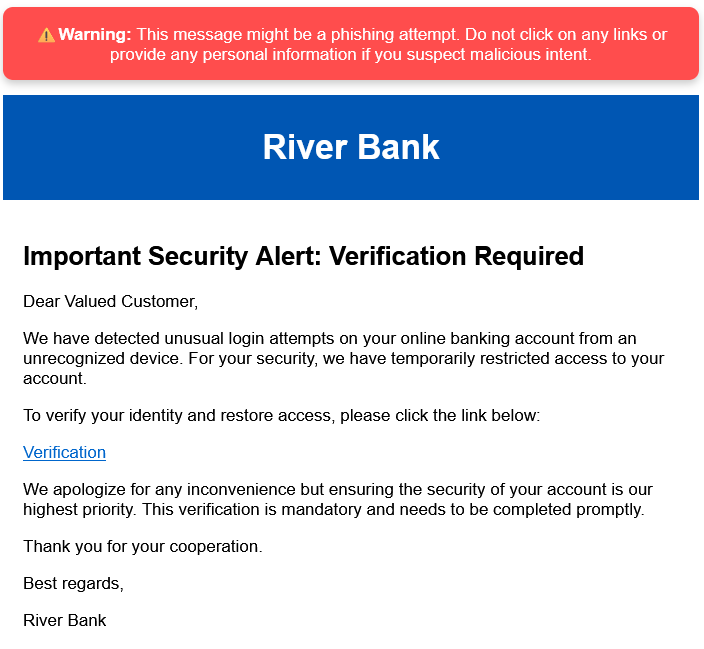
\includegraphics[width=1\linewidth]{figures/banner1_old.png}
  \caption{Variant 1}
\end{subfigure}%
\begin{subfigure}{.5\textwidth}
  \centering
  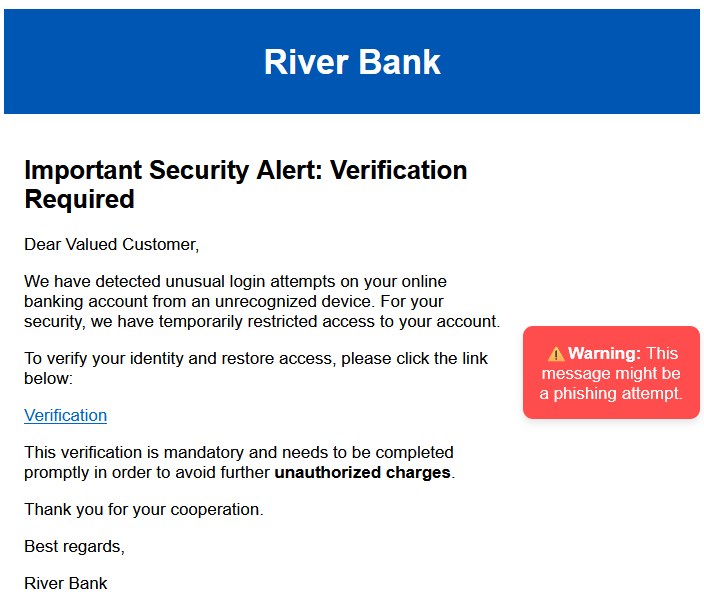
\includegraphics[width=1\linewidth]{figures/banner2_old.png}
  \caption{Variant 2}
\end{subfigure}
\caption{Generic Banner (Version 1)}
\end{figure}

\begin{figure} [H]
\centering
\begin{subfigure}{.5\textwidth}
  \centering
  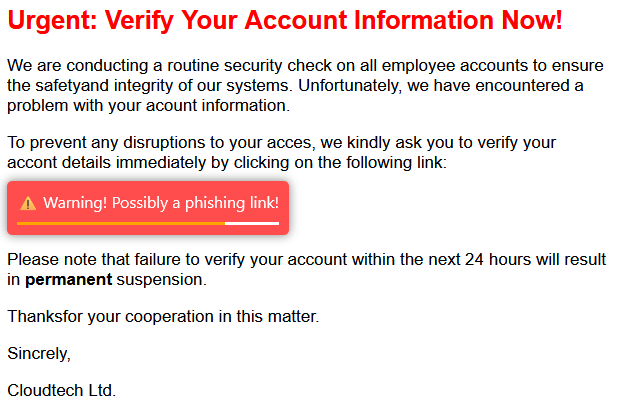
\includegraphics[width=1\linewidth]{figures/hover1_old.png}
  \caption{Variant 1}
\end{subfigure}%
\begin{subfigure}{.5\textwidth}
  \centering
  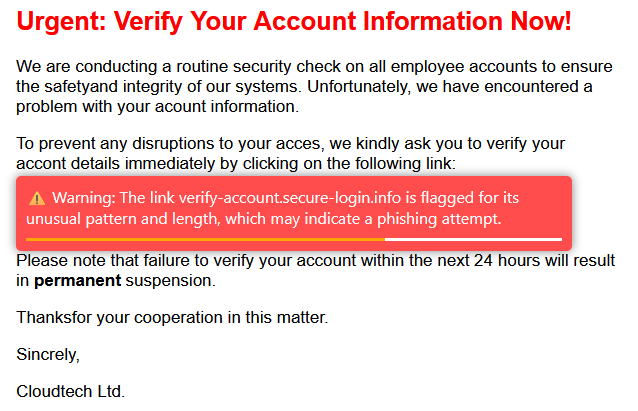
\includegraphics[width=1\linewidth]{figures/hover2_old.png}
  \caption{Variant 2}
\end{subfigure}
\caption{Tooltip Warning on Link Hover (Version 1)}
\end{figure}

\begin{figure} [H]
\centering
\begin{subfigure}{.5\textwidth}
  \centering
  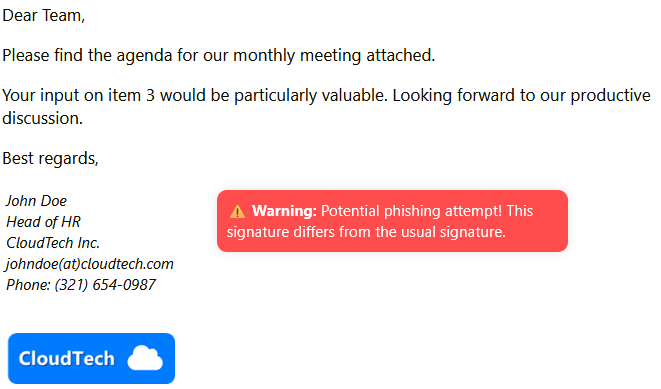
\includegraphics[width=1\linewidth]{figures/sig1_old.png}
  \caption{Variant 1}
\end{subfigure}%
\begin{subfigure}{.5\textwidth}
  \centering
  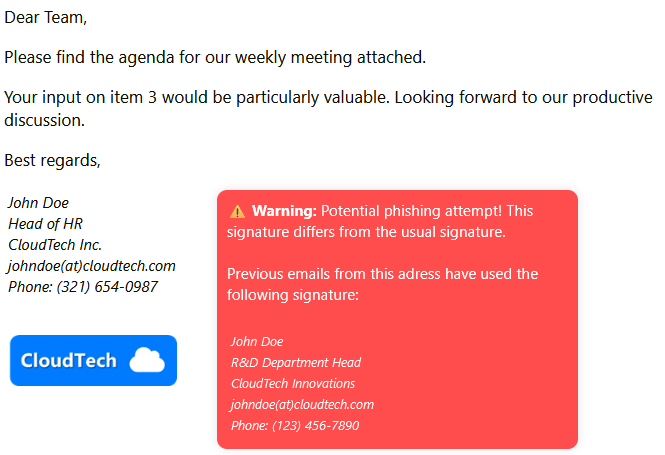
\includegraphics[width=1\linewidth]{figures/sig2_old.png}
  \caption{Variant 2}
\end{subfigure}
\caption{Signature-Specific Warning (Version 1)}
\end{figure}

\begin{figure} [H]
\centering
\begin{subfigure}{.5\textwidth}
  \centering
  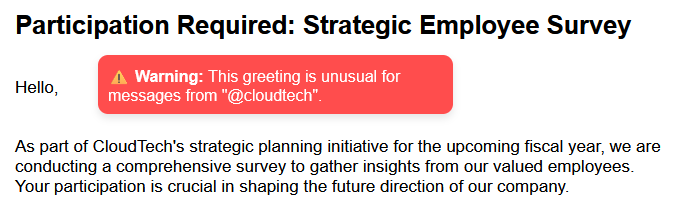
\includegraphics[width=1\linewidth]{figures/greeting1_old.png}
  \caption{Variant 1}
\end{subfigure}%
\begin{subfigure}{.5\textwidth}
  \centering
  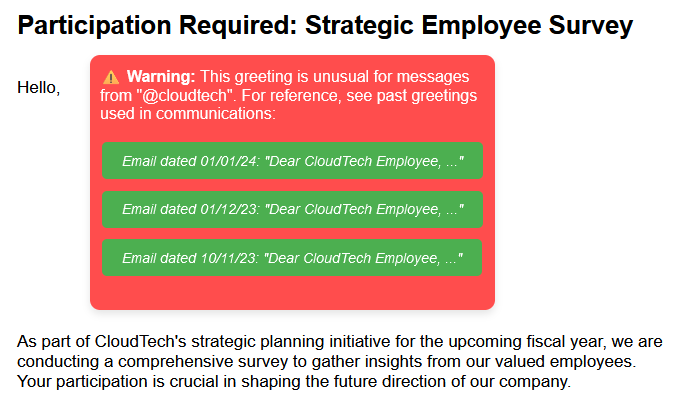
\includegraphics[width=1\linewidth]{figures/greeting2_old.png}
  \caption{Variant 2}
\end{subfigure}
\caption{Greeting-Specific Warning (Version 1)}
\end{figure}

\newpage
\section{QDA Codebook}
\label{sec:qda}
Below is the list of codes developed and utilized during the qualitative data analysis process of our study.
\begin{itemize}
    \item Design Response: This code looks into the overall aesthetic and functional reception of the warning designs by the participants.
    \begin{itemize}
        \item Clarity and Legibility: Evaluates how easily the warnings can be read and understood.
        \item Impact of Animations: Assesses how motion and dynamic elements in the warnings affect user attention and understanding.
        \item Placement: Considers the effectiveness of where warnings are located within the email interface.
        \item Potential Improvements: Gathers participant suggestions on how to enhance the warning designs.
        \item User Attention: Analyzes how conspicuous or inconspicuous these warnings are to the users.
        \begin{itemize}
            \item Conspicuous: Warnings that are immediately noticeable.
            \item  Inconspicuous: Warnings that tend to be overlooked.
        \end{itemize}
    \end{itemize}
    \item Novelties for Participants: Identifies aspects of the phishing warnings that were particularly novel or unexpected to the participants.
    \item Perceived Helpfulness: Explores participants' perception on each warnings helpfulness.
    \begin{itemize}
        \item Negative: Participant feedback that highlights shortcomings or ineffective aspects of the warnings.
        \item Positive: Positive reactions that underscore the effectiveness and utility of the warnings.
        \item Prefered Complexity: Explores participants' preferences for the complexity of the information provided in the warnings.
        \begin{itemize}
            \item More Details: Preference for detailed and informative warnings.
            \item Simplicity: Preference for straightforward, minimal warnings.
        \end{itemize}
    \end{itemize}
\end{itemize}

\newpage
\section{Eye Tracking Heatmap}

\iffalse
\begin{figure}[H]
\centering
\begin{tikzpicture}
\begin{axis}[
    xlabel={Participant ID},
    ylabel={Time to First Fixation (seconds)},
    grid=major,
    xmin=0, xmax=16, 
    ymin=0, ymax=16,  
    xtick={1,2,...,15}, 
    xticklabels={1,2,...,12,13,15,16}, 
    xticklabel style={font=\footnotesize, rotate=0}, 
    yticklabel style={font=\footnotesize}
]
\addplot+[
    only marks,
    mark=*,
    mark size=2.5pt,
    scatter=true, 
    color=blue, 
    fill=blue  
] table [row sep=\\,y=data, x=seq] {
    seq  data\\
    1    2.42\\ 2    0.54\\ 3    1.21\\ 4    0.61\\ 5    2.75\\
    6    0.22\\ 7    1.30\\ 8    1.23\\ 9    2.72\\ 10   1.29\\
    11   1.10\\ 12   0.15\\ 13   2.88\\ 14   1.30\\ 15   15.59\\
};
\end{axis}
\end{tikzpicture}
\caption{Time to first fixation for the top AOI.}
\label{sideaoi}
\end{figure}
\fi

Included here is an eye tracking heatmap using the gaze data of all participants. Although not directly referenced in the main findings, this heatmap may serve as a useful resource for other researchers interested in the visual patterns of user interaction. It also serves an educational purpose, illustrating the application of eye tracking technology in research.

\begin{figure} [ht]
    \centering
    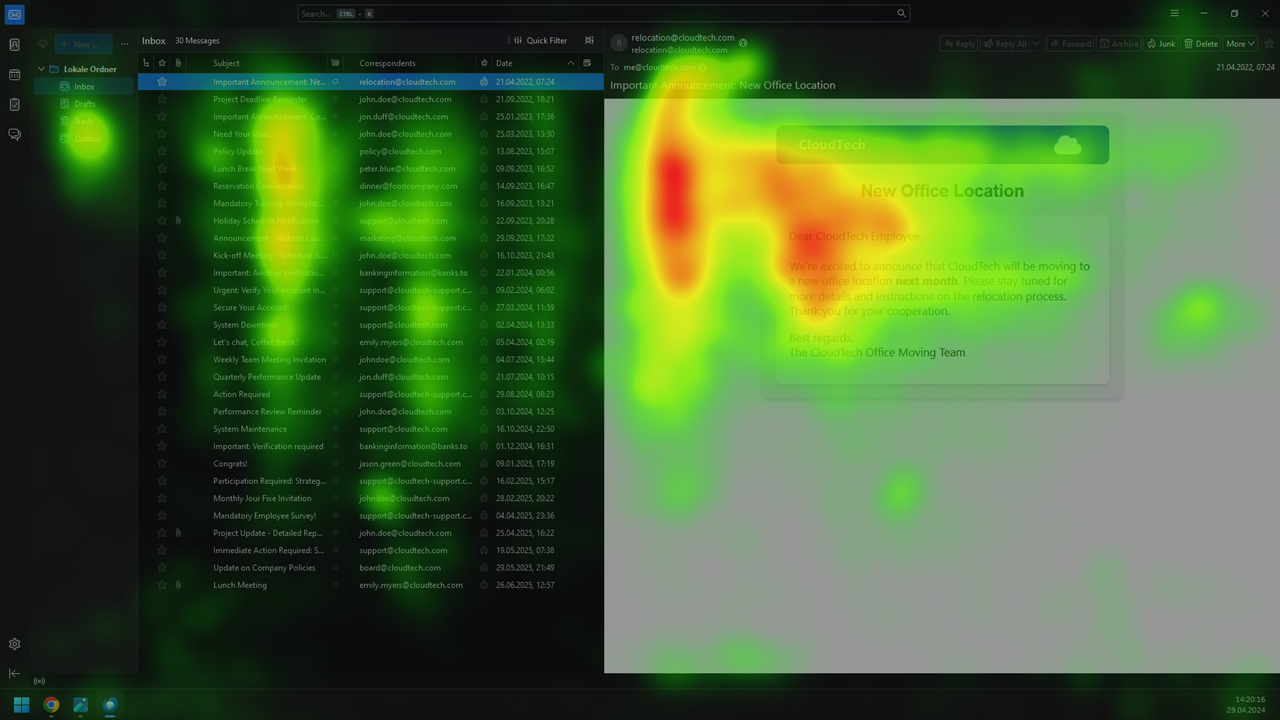
\includegraphics[width=1\linewidth]{figures/heatmap_overlay.png}
    \caption{Accumulated eyetracking heatmap, generated in Tobii Pro Lab}
    \label{fig:heatmap}
\end{figure}

%% !TeX root = main-english.tex
% !TeX spellcheck = en-US
% !TeX encoding = utf8
% -*- coding:utf-8 mod:LaTeX -*-

%This smart spell only works if no changes have been made to the chapter 
%using the options proposed in preambel/chapterheads.tex.
\setchapterpreamble[u]{%
  \dictum[Albert Einstein]{We cannot solve our problems with the same level of thinking that created them}
}
\chapter{LaTeX Hints}
\label{chap:latexhints}

One sentence per line.
This rule is important for the usage of version control systems.
A new line is generated with a blank line.
As you would do in Word:
New paragraphs are generated by pressing enter.
In LaTeX, this does not lead to a new paragraph as LaTeX joins subsequent lines.
In case you want a new paragraph, just press enter twice (!).
This leads to an empty line.
In word, there is the functionality to press shift and enter.
This leads to a hard line break.
The text starts at the beginning of a new line.
In LaTeX, you can do that by using two backslashes (\textbackslash\textbackslash).
This is rarely used.

Please do \textit{not} use two backslahes for new paragraphs.
For instance, this sentence belongs to the same paragraph, whereas the last one started a new one.
A long motivation for that is provided at \url{http://loopspace.mathforge.org/HowDidIDoThat/TeX/VCS/#section.3}.

One can write \emph{emphasized text (rendered in italics)} and \textbf{bold text}.

\section{File Encoding and Support of Umlauts}
\label{sec:firstsectioninlatexhints}
The template offers foll UTF-8 support.
All recent editors should not have issues with that.

\section{Citations}


References are set by means of \texttt{\textbackslash cite[key]}.

\begin{filecontents*}{\democodefile}
Example: \cite{WSPA} or by author input: \citet{WSPA}.
\end{filecontents*}
\PrintDemo{style=parallel}

The following sentence demonstrates
\begin{inparaenum}[1.]
  \item the capitalization of author names at the beginning of the sentence,
  \item the correct citation using author names and the reference,
  \item that the author names are a hyperlink to the bibliography and that
  \item the bibliography contains the name prefix \qq{van der} of \qq{Wil M.\,P.\ van der Aalst}.
\end{inparaenum}

\begin{filecontents*}{\democodefile}
\Citet{RVvdA2016} present a study on the effectiveness of workflow management systems.
\end{filecontents*}
\PrintDemo{style=parallel}

The following sentence demonstrates that you can overwrite the text part of the generated label using \texttt{label} in a bibliopgrahie"=entry, but the year and the uniqueness is still generated by biber.

\begin{filecontents*}{\democodefile}
The workflow engine Apache ODE \cite{ApacheODE} executes \BPEL processes reliably.
\end{filecontents*}
\PrintDemo{style=parallel}

\begin{filecontents*}{\democodefile}
Words are best enclosed using \texttt{\textbackslash qq\{..\}}, then the correct quotes are used.
\end{filecontents*}
\PrintDemo{style=parallel}

When creating the Bibtex file it is recommended to make sure that the DOI is listed.

\section{Formulas and Equations}
\label{sec:mf}

\begin{filecontents*}{\democodefile}
Equations $f(x)=x$ inside the text can be provided.
\end{filecontents*}
\PrintDemo{style=parallel}

A list with all available mathematical symbols is provided at \url{http://texdoc.net/pkg/symbols-a4}.

\begin{filecontents*}{\democodefile}
As example the set of natural numbers is given by $\mathbb{N}$.
\end{filecontents*}
\PrintDemo{style=parallel}

For the documentation of editing mathematical formulas read the package documentation of \texttt{amsmath}\footnote{\url{http://texdoc.net/pkg/amsmath}}.

Equation~\ref{eq:test} is numbered and can be referenced in the text:
\begin{filecontents*}{\democodefile}
\begin{align}
  \label{eq:test}
  x = y
\end{align}
\end{filecontents*}
\PrintDemo{style=parallel}

Following equation is not numbered because of using \texttt{\textbackslash align*} as environment.
\begin{filecontents*}{\democodefile}
\begin{align*}
  x = y
\end{align*}
\end{filecontents*}
\PrintDemo{style=parallel}

The template offers \verb+\abs+ to enable the bars scaling well at the absolute value:

\begin{filecontents*}{\democodefile}
$\abs{X}$.
\end{filecontents*}
\PrintDemo{style=parallel}

More details about mathematical environments provides the documentation available at \url{http://www.ctan.org/tex-archive/help/Catalogue/entries/voss-mathmode.html}.


%%%%%%%%%%%%%%%%%%%%%%%%%%%%%%%%%%%%%%%%%%%%%%%%%%%%%%%%%%%%%%%%%%%%%%%%%%%%%%
\section{Sourcecode}
%%%%%%%%%%%%%%%%%%%%%%%%%%%%%%%%%%%%%%%%%%%%%%%%%%%%%%%%%%%%%%%%%%%%%%%%%%%%%%
\autoref{lst:ListingANDlstlisting} shows how to emmbed source code.
With \texttt{\textbackslash lstinputlisting} the source code can be loaded directly from files.

%Listing-Umgebung wurde durch \newfloat{Listing} definiert
\begin{Listing}
  \begin{lstlisting}
<listing name="second sample">
  <content>not interesting</content>
</listing>
\end{lstlisting}
  \caption{The code is separated by two horizontal lines in the listings environment.}
  \label{lst:ListingANDlstlisting}
\end{Listing}

\begin{filecontents*}{\democodefile}
Source code is also available in the text \lstinline|<listing />|.
\end{filecontents*}
\PrintDemo{style=parallel}


%%%%%%%%%%%%%%%%%%%%%%%%%%%%%%%%%%%%%%%%%%%%%%%%%%%%%%%%%%%%%%%%%%%%%%%%%%%%%%
\section{Pseudocode}
%%%%%%%%%%%%%%%%%%%%%%%%%%%%%%%%%%%%%%%%%%%%%%%%%%%%%%%%%%%%%%%%%%%%%%%%%%%%%%
\autoref{alg:sample} shows a sample algorithm.
\begin{Algorithmus} %Use the environment only if you want to place the algorithm similar to graphics from TeX
  \caption{Sample algorithm}
  \label{alg:sample}
  \begin{algorithmic}
\Procedure{Sample}{$a$,$v_e$}
\State $\mathsf{parentHandled} \gets (a = \mathsf{process}) \lor \mathsf{visited}(a'), (a',c,a) \in \mathsf{HR}$
\State \Comment $(a',c'a) \in \mathsf{HR}$ denotes that $a'$ is the parent of $a$
\If{$\mathsf{parentHandled}\,\land(\mathcal{L}_\mathit{in}(a)=\emptyset\,\lor\,\forall l \in \mathcal{L}_\mathit{in}(a): \mathsf{visited}(l))$}
\State $\mathsf{visited}(a) \gets \text{true}$
\State $\mathsf{writes}_\circ(a,v_e) \gets
\begin{cases}
\mathsf{joinLinks}(a,v_e) & \abs{\mathcal{L}_\mathit{in}(a)} > 0\\
\mathsf{writes}_\circ(p,v_e)
& \exists p: (p,c,a) \in \mathsf{HR}\\
(\emptyset, \emptyset, \emptyset, false) & \text{otherwise}
\end{cases}
$
\If{$a\in\mathcal{A}_\mathit{basic}$}
  \State \Call{HandleBasicActivity}{$a$,$v_e$}
\ElsIf{$a\in\mathcal{A}_\mathit{flow}$}
  \State \Call{HandleFlow}{$a$,$v_e$}
\ElsIf{$a = \mathsf{process}$} \Comment Directly handle the contained activity
  \State \Call{HandleActivity}{$a'$,$v_e$}, $(a,\bot,a') \in \mathsf{HR}$
  \State $\mathsf{writes}_\bullet(a) \gets \mathsf{writes}_\bullet(a')$
\EndIf
\ForAll{$l \in \mathcal{L}_\mathit{out}(a)$}
  \State \Call{HandleLink}{$l$,$v_e$}
\EndFor
\EndIf
\EndProcedure
  \end{algorithmic}
\end{Algorithmus}

\clearpage
And if you want to write an algorithm that goes over several pages, you can only do this with the following \textbf{dirty} hack:

{
\begin{minipage}{\textwidth}
  \hrule height .8pt width\textwidth
  \vskip.3em%\vskip\abovecaptionskip\relax
  \stepcounter{Algorithmus}
  \addcontentsline{alg}{Algorithmus}{\protect\numberline{\theAlgorithmus}{\ignorespaces Description \relax}}
  \noindent\textbf{Algorithmus \theAlgorithmus} Description
  %\stepcounter{algorithm}
  %\addcontentsline{alg}{Algorithmus}{\thealgorithm{}\hskip0em Description}
  %\textbf{Algorithmus \thealgorithm} Description
  \vskip.3em%\vskip\belowcaptionskip\relax
  \hrule height .5pt width\textwidth
\end{minipage}
%without the following line, the text is nerer at the rule
\vskip-.3em
%
code goes here\\
test2\\
%
\vskip-.7em
\hrule height .5pt width\textwidth
}


%%%%%%%%%%%%%%%%%%%%%%%%%%%%%%%%%%%%%%%%%%%%%%%%%%%%%%%%%%%%%%%%%%%%%%%%%%%%%%
\section{Figures}
%%%%%%%%%%%%%%%%%%%%%%%%%%%%%%%%%%%%%%%%%%%%%%%%%%%%%%%%%%%%%%%%%%%%%%%%%%%%%%
The \autoref{fig:chor1} and \ref{fig:chor2} are important to understand this document.
In the appendix \vref{fig:AnhangsChor} shows again the complete choreography.

%The parameters in square brackets are optional - e.g. [htb!]
%htb! means: Dear LaTeX, please place this image here first ("_h_ere"). If this does not work, place it at the "_t_op" of the page. And if this is not possible, please place it at the "_b_ottom" of the page. And please, please prefer here and above, even if it doesn't look so optimal ("!")
%These should NOT be used if possible. LaTeX's algorithm for placing the glide environment is already very good!
\begin{figure}
  \centering
  \includegraphics[width=\textwidth]{choreography.pdf}
  \caption{Example Choreography}
  \label{fig:chor1}
\end{figure}

\begin{figure}
  \centering
  \includegraphics[width=.8\textwidth]{choreography.pdf}
  \caption[Example Choreography]{The example choreography. Now slightly smaller to demonstrate \texttt{\textbackslash textwidth}. And also the use of alternative captions for the list of images. However, the latter is only conditionally recommended, because who reads so much text under a picture? Or is it just a matter of style?}
  \label{fig:chor2}
\end{figure}


\begin{figure}
  \hfill
  \begin{subfigure}{.3\textwidth}
    \includegraphics[width=\textwidth]{choreography.pdf}
    \caption{Choreography 1}
    \label{fig:subfigA}
  \end{subfigure}
  \hfill
  \begin{subfigure}{.3\textwidth}
    \includegraphics[width=\textwidth]{choreography.pdf}
    \caption{Choreography 2}
    \label{fig:subfigB}
  \end{subfigure}
  \hfill
  \begin{subfigure}{.3\textwidth}
    \includegraphics[width=.9\textwidth]{choreography.pdf}
    \caption{Choreography 3}
    \label{fig:subfigC}
  \end{subfigure}
  \caption{Example to place 3 illustrations next to each other. Further, it is possible to reference each separately.}
  \label{fig:subfig_example}
\end{figure}

\autoref{fig:subfig_example} shows the usage of the package subcaption.
It is indeed possible to reference to sub figures: \autoref{fig:subfigA}.

It is possible to convert SVGs to PDF directly during compilation.
This is described in the source code of latex-tipps.tex, but commented out.

\iffalse % <-- Take this away if inkscape is in the path
  The SVG in \autoref{fig:directSVG} is directly included, while the text in the SVG in \autoref{fig:latexSVG} is set using pdflatex.
  If you want to see the graphics, inkscape must be in PATH and in the text source \texttt{\textbackslash{}iffalse} and \text{\textbackslash{}iftrue} have to be commented out.

  \begin{figure}
    \centering
    \includegraphics{svgexample.svg}
    \caption{SVG directly included}
    \label{fig:directSVG}
  \end{figure}

  \begin{figure}
    \centering
    \def\svgwidth{.4\textwidth}
    \includesvg{svgexample}
    \caption{Text in SVN set via \LaTeX{}}
    \label{fig:latexSVG}
  \end{figure}
\fi % <-- Take this away if inkscape is in the path



\section{More Illustrations}
\autoref{fig:AnhangsChor,fig:AnhangsChor2} show two choreographies, which should further explain the facts. The second figure is rotated 90 degrees to demonstrate the \texttt{pdflscape} package.

\begin{figure}
  \centering
  \includegraphics[width=\textwidth]{choreography.pdf}
  \caption{Example Choreography I}
  \label{fig:AnhangsChor}
\end{figure}

\begin{landscape}
  %sidewaysfigure
  \begin{figure}
    \centering
    \includegraphics[width=\textwidth]{choreography.pdf}
    \caption{Example Choreography II}
    \label{fig:AnhangsChor2}
  \end{figure}
\end{landscape}


\IfFileExists{pgfplots.sty}{
  %%%%%%%%%%%%%%%%%%%%%%%%%%%%%%%%%%%%%%%%%%%%%%%%%%%%%%%%%%%%%%%%%%%%%%%%%%%%%%
  \section{Plots with pgfplots}
  %%%%%%%%%%%%%%%%%%%%%%%%%%%%%%%%%%%%%%%%%%%%%%%%%%%%%%%%%%%%%%%%%%%%%%%%%%%%%%
  The package pdfplots provides plotting of functions directly in \LaTeX~like with matlab or gnuplot. Some visual examples are available here\footnote{\url{http://texdoc.net/pkg/visualtikz}}.
  \begin{figure}[h]
    \centering
    \begin{tikzpicture}
      \begin{axis}[xlabel=$x$,
          ylabel=$\sin(x)$]
        \addplot {sin(deg(x))};  % Print sine function
      \end{axis}
    \end{tikzpicture}
    \caption{Plot of $\sin(x)$ direclty inside the figure environment with pgfplots.}
  \end{figure}

  \begin{figure}[h]
    \centering
    \begin{tikzpicture}
      \begin{axis}[xlabel=$x$,
          ylabel=$y$]
        \addplot table [x=a, y=c, col sep=comma] {data/data.csv};  % Read coordinates from csv file and plot them
      \end{axis}
    \end{tikzpicture}
    \caption{Coordinates $x$ and $y$ read from csv file and plotted pgfplots.}
  \end{figure}

}{}


%%%%%%%%%%%%%%%%%%%%%%%%%%%%%%%%%%%%%%%%%%%%%%%%%%%%%%%%%%%%%%%%%%%%%%%%%%%%%%
\section{Figures with tikz}
%%%%%%%%%%%%%%%%%%%%%%%%%%%%%%%%%%%%%%%%%%%%%%%%%%%%%%%%%%%%%%%%%%%%%%%%%%%%%%
The tikz is a package for creating graphics programmatically. With this package grids or other regular strucutres can be easliy generated.

\begin{figure}[ht]
  \centering
  \begin{tikzpicture}
    \draw(0,0) rectangle (4,4);
    \foreach \x in {0.5,1,1.5,2,2.5,3,3.5}
    \foreach \y in {0.5,1,1.5,2,2.5,3,3.5}
    \draw(\x,\y) circle (1pt);
  \end{tikzpicture}
  \caption{A regular grid genrated with easily with two for loops.}\label{fig:tikz_example}
\end{figure}


%%%%%%%%%%%%%%%%%%%%%%%%%%%%%%%%%%%%%%%%%%%%%%%%%%%%%%%%%%%%%%%%%%%%%%%%%%%%%%
\section{UML diagrams using tikz-uml}
%%%%%%%%%%%%%%%%%%%%%%%%%%%%%%%%%%%%%%%%%%%%%%%%%%%%%%%%%%%%%%%%%%%%%%%%%%%%%%

\autoref{fig:uml} presents a class diagram typeset using tikz-uml.

\begin{figure}
  \centering
  \begin{tikzpicture}
  \begin{umlpackage}{p}
  \begin{umlpackage}{sp1}
  \umlclass[template=T]{A}{
    n : uint \\ t : float
  }{}
  \umlclass[y=-3]{B}{
    d : double
  }{
    \umlvirt{setB(b : B) : void} \\ getB() : B}
  \end{umlpackage}
  \begin{umlpackage}[x=10,y=-6]{sp2}
  \umlinterface{C}{
    n : uint \\ s : string
  }{}
  \end{umlpackage}
  \umlclass[x=2,y=-10]{D}{
    n : uint
    }{}
  \end{umlpackage}

  \umlassoc[geometry=-|-, arg1=tata, mult1=*, pos1=0.3, arg2=toto, mult2=1, pos2=2.9, align2=left]{C}{B}
  \umlunicompo[geometry=-|, arg=titi, mult=*, pos=1.7, stereo=vector]{D}{C}
  \umlimport[geometry=|-, anchors=90 and 50, name=import]{sp2}{sp1}
  \umlaggreg[arg=tutu, mult=1, pos=0.8, angle1=30, angle2=60, loopsize=2cm]{D}{D}
  \umlinherit[geometry=-|]{D}{B}
  \umlnote[x=2.5,y=-6, width=3cm]{B}{A note with respect to class B}
  \umlnote[x=7.5,y=-2]{import-2}{A anotation}
  \end{tikzpicture}
  \caption{Class diagram generated with tikz-uml. Example adapted from Nicolas Kielbasiewicz.}
  \label{fig:uml}
\end{figure}

\section{UML diagrams using PlantUML}

In case \lualatex{} is used and PlantUML is installed, UML diagrams can be defined using PlantUML.

% Only works if "--shell-escape" is activated. Please activate only if you are sure, your compilation settings are correct
%\IfFileExists{plantuml.sty}{\input{latexhints-english-plantuml}}{}


%%%%%%%%%%%%%%%%%%%%%%%%%%%%%%%%%%%%%%%%%%%%%%%%%%%%%%%%%%%%%%%%%%%%%%%%%%%%%%
\section{Linguistic Forests}
%%%%%%%%%%%%%%%%%%%%%%%%%%%%%%%%%%%%%%%%%%%%%%%%%%%%%%%%%%%%%%%%%%%%%%%%%%%%%%

\begin{filecontents*}{\democodefile}
\begin{forest}
  [VP
    [DP]
    [V’
      [V]
      [DP]
    ]
  ]
\end{forest}
\end{filecontents*}
\PrintDemo{style=parallel}


%%%%%%%%%%%%%%%%%%%%%%%%%%%%%%%%%%%%%%%%%%%%%%%%%%%%%%%%%%%%%%%%%%%%%%%%%%%%%%
\section{Tables}
%%%%%%%%%%%%%%%%%%%%%%%%%%%%%%%%%%%%%%%%%%%%%%%%%%%%%%%%%%%%%%%%%%%%%%%%%%%%%%
\autoref{tab:Ergebnisse} shows results and \autoref{tab:Werte} shows how numerical data can be represented in a table.
\begin{table}
  \centering
  \begin{tabular}{ccc}
    \toprule
    \multicolumn{2}{c}{\textbf{summed}} & \textbf{Title}                                                          \\ \midrule
    Table                                      & as                                                           & in      \\
    \url{tabsatz.pdf}                            & recommended                                                     & gesetzt \\

    \multirow{2}{*}{Example}                    & \multicolumn{2}{c}{a nice example}                                \\
                                                 & \multicolumn{2}{c}{for using \qq{multirow}}           \\
    \bottomrule
  \end{tabular}
  \caption[Example Table]{Exampe Table -- see \url{http://www.ctan.org/tex-archive/info/german/tabsatz/}}
  \label{tab:Ergebnisse}
\end{table}

\begin{table}
  \centering
  \begin{tabular}{l *{8}{d{3.2}}}
    \toprule

                         & \multicolumn{2}{c}{\textbf{Parameter 1}} & \multicolumn{2}{c}{\textbf{Parameter 2}} & \multicolumn{2}{c}{\textbf{Parameter 3}} & \multicolumn{2}{c}{\textbf{Parameter 4}}                                                                                                                                       \\
    \cmidrule(r){2-3}\cmidrule(lr){4-5}\cmidrule(lr){6-7}\cmidrule(l){8-9}

    \textbf{Bedingungen} & \multicolumn{1}{c}{\textbf{M}}           & \multicolumn{1}{c}{\textbf{SD}}          & \multicolumn{1}{c}{\textbf{M}}           & \multicolumn{1}{c}{\textbf{SD}}          & \multicolumn{1}{c}{\textbf{M}} & \multicolumn{1}{c}{\textbf{SD}} & \multicolumn{1}{c}{\textbf{M}} & \multicolumn{1}{c}{\textbf{SD}} \\
    \midrule

    W                    & 1.1                                      & 5.55                                     & 6.66                                     & .01                                      &                                &                                 &                                &                                 \\
    X                    & 22.22                                    & 0.0                                      & 77.5                                     & .1                                       &                                &                                 &                                &                                 \\
    Y                    & 333.3                                    & .1                                       & 11.11                                    & .05                                      &                                &                                 &                                &                                 \\
    Z                    & 4444.44                                  & 77.77                                    & 14.06                                    & .3                                       &                                &                                 &                                &                                 \\
    \bottomrule
  \end{tabular}

  \caption{Example table for 4 constraints (W-Z), each having 4 parameters with (M und SD). Note: use always the same number of decimal places.}
  \label{tab:Werte}
\end{table}

\IfFileExists{pgfplotstable.sty}{

\subsection{Tables with pgfplots}
With the pgfplotstable package tables can be directly generated from a csv file.

\begin{table}[h]
\centering
\pgfplotstabletypeset[
col sep = comma,
every head row/.style={before row=\toprule,after row=\midrule},
every last row/.style={after row=\bottomrule},
display columns/0/.style={string type,column name={}}
]
{data/data.csv}
\caption{Table direclty generated from the values of a csf file.}
\end{table}
}{}


\section{Tables spanning multiple pages}


\begin{longtable}{|l|l|l|}
\caption{A sample long table.} \label{tab:long} \\

\hline \multicolumn{1}{|c|}{\textbf{First column}} & \multicolumn{1}{c|}{\textbf{Second column}} & \multicolumn{1}{c|}{\textbf{Third column}} \\ \hline
\endfirsthead

\multicolumn{3}{c}%
{{\bfseries \tablename\ \thetable{} -- continued from previous page}} \\
\hline \multicolumn{1}{|c|}{\textbf{First column}} & \multicolumn{1}{c|}{\textbf{Second column}} & \multicolumn{1}{c|}{\textbf{Third column}} \\ \hline
\endhead

\hline \multicolumn{3}{|r|}{{Continued on next page}} \\ \hline
\endfoot

\hline \hline
\endlastfoot

A & BC & D \\
A & BC & D \\
A & BC & D \\
A & BC & D \\
A & BC & D \\
A & BC & D \\
A & BC & D \\
A & BC & D \\
A & BC & D \\
A & BC & D \\
A & BC & D \\
A & BC & D \\
A & BC & D \\
A & BC & D \\
A & BC & D \\
A & BC & D \\
A & BC & D \\
A & BC & D \\
A & BC & D \\
A & BC & D \\
A & BC & D \\
A & BC & D \\
A & BC & D \\
A & BC & D \\
A & BC & D \\
A & BC & D \\
A & BC & D \\
A & BC & D \\
A & BC & D \\
A & BC & D \\
A & BC & D \\
A & BC & D \\
A & BC & D \\
A & BC & D \\
A & BC & D \\
A & BC & D \\
A & BC & D \\
A & BC & D \\
A & BC & D \\
A & BC & D \\
A & BC & D \\
A & BC & D \\
A & BC & D \\
A & BC & D \\
A & BC & D \\
A & BC & D \\
A & BC & D \\
A & BC & D \\
A & BC & D \\
A & BC & D \\
A & BC & D \\
A & BC & D \\
A & BC & D \\
A & BC & D \\
A & BC & D \\
A & BC & D \\
A & BC & D \\
A & BC & D \\
A & BC & D \\
A & BC & D \\
A & BC & D \\
A & BC & D \\
A & BC & D \\
A & BC & D \\
A & BC & D \\
A & BC & D \\
A & BC & D \\
A & BC & D \\
A & BC & D \\
A & BC & D \\
A & BC & D \\
A & BC & D \\
A & BC & D \\
A & BC & D \\
A & BC & D \\
A & BC & D \\
A & BC & D \\
A & BC & D \\
A & BC & D \\
A & BC & D \\
\end{longtable}


%%%%%%%%%%%%%%%%%%%%%%%%%%%%%%%%%%%%%%%%%%%%%%%%%%%%%%%%%%%%%%%%%%%%%%%%%%%%%%
\section{Abbreviations}
%%%%%%%%%%%%%%%%%%%%%%%%%%%%%%%%%%%%%%%%%%%%%%%%%%%%%%%%%%%%%%%%%%%%%%%%%%%%%%
At the first pass the \gls{fr} was 5.
At the second pass was \gls{fr} 3.
The plural form can be seen here: \glspl{er}.
To demonstrate what the list of abbreviations looks like for longer description texts, \glspl{rdbms} must be mentioned here.

With \verb+\gls{...}+ you can enter abbreviations, the first time you call it, the long form is used.
When reusing \verb+\gls{..}+ the short form is automatically displayed.
The abbreviation is also automatically inserted in the abbreviation list.
With \verb+\glspl{...}+ the plural form is used.
If you want the short form to appear directly at the first use, you can use \verb+\glsunset{..}+ to mark an abbreviation as already used.
The opposite is achieved with \verb+\glsreset{..}+.

Abbreviations are defined in \verb+\content\ausarbeitung.tex+ by means of \verb+\newacronym{...}{...}{...}+.

More information at: \url{http://tug.ctan.org/macros/latex/contrib/glossaries/glossariesbegin.pdf}
%%%%%%%%%%%%%%%%%%%%%%%%%%%%%%%%%%%%%%%%%%%%%%%%%%%%%%%%%%%%%%%%%%%%%%%%%%%%%%
\section{References}
%%%%%%%%%%%%%%%%%%%%%%%%%%%%%%%%%%%%%%%%%%%%%%%%%%%%%%%%%%%%%%%%%%%%%%%%%%%%%%
For distant sections \qq{varioref} is recommended:
\qq{See \vref{sec:mf}}.
The command \texttt{\textbackslash{}vref} works similar to \texttt{\textbackslash{}cref} the difference beeing that a reference to the page is additionally added.
\texttt{vref}: \qq{\vref{sec:firstsectioninlatexhints}}, \texttt{cref}: \qq{\autoref{sec:firstsectioninlatexhints}}, \texttt{ref}: \qq{\ref{sec:firstsectioninlatexhints}}.

If \qq{varioref} causes difficulties, then \qq{cref} can be used instead.
This also creates the word \qq{section} automatically: \autoref{sec:mf}.
This is also possible for illustrations etc.
In English please use \verb1\autoref{...}1 (with large \qq{C} at the beginning).

%With MiKTeX installation from 2012-01-16 no longer necessary.
%If a section becomes longer than one page and you want to refer to a specific place in the section with \texttt{\textbackslash{}vref}, then you should use \texttt{\textbackslash{}phantomsection} then using \texttt{vref} will also display the correct page number.

%%The link location will be placed on the line below.
%%Tipp von http://en.wikibooks.org/wiki/LaTeX/Labels_and_Cross-referencing#The_hyperref_package_and_.5Cphantomsection
%\phantomsection
%\label{alabel}
%View the example for \texttt{\textbackslash{}phantomsection} in the \LaTeX{} source code.

%Here is the example: See Section \vref{hack1} and Section \vref{hack2}.
%%%%%%%%%%%%%%%%%%%%%%%%%%%%%%%%%%%%%%%%%%%%%%%%%%%%%%%%%%%%%%%%%%%%%%%%%%%%%%
\section{Definitions}
%%%%%%%%%%%%%%%%%%%%%%%%%%%%%%%%%%%%%%%%%%%%%%%%%%%%%%%%%%%%%%%%%%%%%%%%%%%%%%
\begin{definition}[Title]
  \label{def:def1}
  Definition Text
\end{definition}

\autoref{def:def1} shows \ldots

%%%%%%%%%%%%%%%%%%%%%%%%%%%%%%%%%%%%%%%%%%%%%%%%%%%%%%%%%%%%%%%%%%%%%%%%%%%%%%
\section{Footnotes}
%%%%%%%%%%%%%%%%%%%%%%%%%%%%%%%%%%%%%%%%%%%%%%%%%%%%%%%%%%%%%%%%%%%%%%%%%%%%%%
Footnotes are provided by the command \verb+\footnote{...}+\footnote{\label{fussnote}Example footnote.}. Citing footnotes is possible by provinding a label\verb+\footnote{\label{...}...}+ and cite the footnote with \verb+\autoref{...}+ in the text\autoref{fussnote}.
%%%%%%%%%%%%%%%%%%%%%%%%%%%%%%%%%%%%%%%%%%%%%%%%%%%%%%%%%%%%%%%%%%%%%%%%%%%%%%

%%%%%%%%%%%%%%%%%%%%%%%%%%%%%%%%%%%%%%%%%%%%%%%%%%%%%%%%%%%%%%%%%%%%%%%%%%%%%%
\section{Various Things}
%%%%%%%%%%%%%%%%%%%%%%%%%%%%%%%%%%%%%%%%%%%%%%%%%%%%%%%%%%%%%%%%%%%%%%%%%%%%%%
\label{sec:diff}
\ifdeutsch
  Numbers (123\,654\,789) are nicely set.
  Either in a line or as non-lining figure.
  The latter is reached by parameter \texttt{osf} at package \texttt{libertine} or.\ \texttt{mathpazo} in \text{fonts.tex}.
\fi

\begin{filecontents*}{\democodefile}
\begin{compactenum}[I.]
  \item You can also keep the numbering compact thanks to paralist
  \item and switch to a different numbering
\end{compactenum}
\end{filecontents*}
\PrintDemo{style=parallel}

The words \qq{workflow} and \qq{dwarflike} can be copied from the PDF and pasted to a text file.

\begin{filecontents*}{\democodefile}
In case \LuaLaTeX{} is used as compiler, there is no ligature at \qq{f\/l} in the word \qq{dwarflike} (in contrast to \qq{fl} at \qq{workflow}).
In other words: \qq{dwarflike} and \qq{dwarf\/like} look the same in the PDF.
In case they do not, there is an issue with Lua\LaTeX{} and the selnolig package.
\end{filecontents*}
\PrintDemo{style=parallel}
% Meta comment: The precise form of the optimal ligation suppression command may vary depending on the character pairs involved - see https://tex.stackexchange.com/q/28437/9075


%%%%%%%%%%%%%%%%%%%%%%%%%%%%%%%%%%%%%%%%%%%%%%%%%%%%%%%%%%%%%%%%%%%%%%%%%%%%%%
\section{Closing remarks}
%%%%%%%%%%%%%%%%%%%%%%%%%%%%%%%%%%%%%%%%%%%%%%%%%%%%%%%%%%%%%%%%%%%%%%%%%%%%%%
Please feel free to provide enhancements for this template and create a new ticket on GitHub (\url{https://github.com/latextemplates/uni-stuttgart-computer-science-template/issues}).


\pagestyle{empty}
\renewcommand*{\chapterpagestyle}{empty}
\Affirmation
\end{document}
